\documentclass[11pt]{article}
\usepackage{geometry}                % See geometry.pdf to learn the layout options. There are lots.
\geometry{letterpaper}                   % ... or a4paper or a5paper or ... 
%\geometry{landscape}                % Activate for for rotated page geometry
%\usepackage[parfill]{parskip}    % Activate to begin paragraphs with an empty line rather than an indent
\usepackage{graphicx}
\usepackage{amssymb}
\usepackage{epstopdf}
\usepackage{hyperref} %url
\usepackage{xurl} %break in urls, but included only in recent versions of MacTex
\usepackage{float} % [H] as figure position
\usepackage{authblk} %authors and affiliations
\usepackage{fancyvrb} %to use Verbatim
\usepackage{booktabs} % for tabular rules
\usepackage{verbatim} %to use \begin{comment} \end{comment}
\usepackage[round]{natbib}
\usepackage[super]{nth}  %days in dates
\usepackage{t1enc} % << e >>


% to insert DRAFT at the beginning of each page
% http://ctan.mirror.garr.it/mirrors/CTAN/info/italian/fancyhdr/itfancyhdr.pdf
\usepackage{fancyhdr}
\pagestyle{fancy}
\lhead{}
\rhead{}
\chead{Work in progress \& draft: Comments and Corrections Welcome!}

\DeclareGraphicsRule{.tif}{png}{.png}{`convert #1 `dirname #1`/`basename #1 .tif`.png}

\begin{document}

\title{The Contagion Sequences of the Epidemic S.I.s.a.R. Model: a Source of Suggestions for Intervention Policies}
%\author{Gianpiero Pescarmona, Pietro Terna,  Alberto Acquadro, Paolo Pescarmona,\\ Giuseppe Russo, and Stefano Terna}
\author[1]{Gianpiero Pescarmona}
\author[2]{Pietro Terna}
\author[1]{Alberto Acquadro}
\author[3]{Paolo Pescarmona}
\author[4]{Giuseppe Russo}
\author[5]{Stefano Terna}

\renewcommand\Affilfont{\itshape\small}
\affil[1]{University of Torino, Italy}
\affil[2]{University of Torino, Italy, retired; Fondazione Collegio Carlo Alberto, Torino, Italy\footnote{Corresponding author, \url{mailto:pietro.terna@unito.it}}}
\affil[3]{University of Groningen, The Netherlands}
\affil[4]{Centro Einaudi, Torino, Italy}
\affil[5]{TomorrowData\footnote{\url{https://tomorrowdata.io}}}


\date{\today}                                           % Activate to display a given date or no date

\maketitle

\begin{abstract}
 
We propose an agent-based model to simulate the Covid-19 epidemic diffusion, with Susceptible, Infected, symptomatic, asymptomatic, and Recovered people: hence the name S.I.s.a.R. The scheme comes from S.I.R. models, with (i) infected agents categorized as symptomatic and asymptomatic and (ii) the places of contagion specified in a detailed way, thanks to agent-based modeling capabilities. The model includes Piedmont's structural data, an Italian region, but it can be readily calibrated it for other areas. The model reproduces a realistic calendar (e.g., national or local government decisions), via its script interpreter. 

The model allows analyzing the sequences of contagions in simulated epidemics, while taking in account the places where they occur. We represent each infecting agent as a horizontal segment with a vertical connection to another agent receiving the infection. We represent the second agent via a further segment at an upper layer. With colors, line thickness, and styles, we display multiple data. This enables understanding at a glance how an epidemic episode is developing. In this way, it is easier to reason about countermeasures and, thus, to develop intervention policies.

 
\end{abstract}

\section{A quick introduction to epidemic modeling}

The starting point from which we built our model is that of S.I.R compartmental models with Susceptible, Infected, and Recovered people. This approach allows looking at the epidemic dynamics, but on a macro scale. While the Covid-19 epidemic was spreading, there have been several attempts to introduce more realistic compartmental subdivisions. A relevant example in this direction is that of \cite{Scala:2020aa}. The research also been followed other work lines, as in \cite{doi:10.1142/S0218202520500323}, where a multiscale framework accounts for the interaction of different spatial levels, from the small scale of the virus itself and cells, to the large scale of individuals and further up to the collective behavior of populations.

Following \cite{rahmandad2008heterogeneity}, we know that the analysis based on the assumption of  heterogeneity strongly differs from S.I.R. compartmental structures modeled by differential equations. Their work ponders when it is better to use agent-based models and when it would be better to use differential equation models. Differential equation models assume homogeneity and perfect mixing within compartments, while agent-based models can capture heterogeneity in agent attributes and the structure of their interactions. We follow the second approach.

Finally, we subscribe the call of \cite{squazzoni2020} to <<cover the full behavioural and social complexity of societies under pandemic crisis>> and we move in that directionin our work reported here.


\subsection{Why model? Why agents? Why another model? }

Why another model, and most of all, with \cite{epstein2008model}, why model? With the author, the reply is: 
\begin{quote}
The choice (\ldots) is not whether to build models; it's whether to build explicit ones. In explicit models, assumptions are laid out in detail, so we can study exactly what they entail. On these assumptions, this sort of thing happens. When you alter the assumptions that is what happens. By writing explicit models, you let others replicate your results.
\end{quote}

And, strongly:
\begin{quote} 
I am always amused when these same people challenge me with the question,``Can you validate your model'' The appropriate retort, of course, is,``Can you validate yours?'' At least I can write mine down so that it can, in principle, be calibrated to data, if that is what you mean by ``validate'' a term I assiduously avoid.
\end{quote}

To reply to ``why agents?'', with \cite{axtell2000agents} we define in short what an agent-based model is:
\begin{quote} 
An agent-based model consists of individual agents, commonly implemented in software as objects. Agent objects have states and rules of behavior. Running such a model simply amounts to instantiating an agent population, letting the agents interact, and monitoring what happens. That is, executing the model---spinning it forward in time---is all that is necessary in order to ``solve'' it.
\end{quote}

More in detail:
\begin{quote} 
There are, ostensibly, several advantages of agent-based computational modeling over conventional mathematical theorizing. First, as described above, it is easy to limit agent rationality in agent-based computational models. Second, even if one wishes to use completely rational agents, it is a trivial matter to make agents heterogeneous in agent-based models. One simply instantiates a population having some distribution of initial states, e.g., preferences. That is, there is no need to appeal to representative agents. Third, since the model is ``solved'' merely by executing it, there results an entire dynamical history of the process under study. That is, one need not focus exclusively on the equilibria, should they exist, for the dynamics are an inescapable part of running the agent model. Finally, in most social processes either physical space or social networks matter. These are difficult to account for mathematically except in highly stylized ways. However, in agent-based models it is usually quite easy to have the agent interactions mediated by space or networks or both.
\end{quote}

And now, "why another?" As a commitment to our creativity, using our knowledge to understand what is happening. Indeed, with arbitrariness: it is up to others and time to judge. Modeling the Covid-19 pandemic requires a scenario and the actors.
As in every play, the author defines the roles of the actors and the environment. The characters are not real, they are pre-built by the author, and they act according to their peculiar constraints. If the play is successful, they will play for a long time, even centuries. If not, we will rapidly forget them. Shakespeare Hamlet is still playing after centuries, even if he is entirely imaginary.

The same holds for our simulations: we are the authors, we arbitrarily define the characters, we force them to act again and again in different scenarios. In both plays and simulations, we compress the time: whole life to 2 or 3 hours on the stage. In a few seconds, we run the Covid-19 pandemic spread in a given regional area.

\subsection{Our model}

With our model, we move from a macro compartmental vision to a meso and microanalysis capability. Its main characteristics are:

\begin{itemize}

\item
scalability: we take in account the interactions between virus and molecules inside the host, the interactions between individuals in more or less restricted contexts, the movement between different environments (home, school, workplace, open spaces, shops, \ldots);\footnote{In a second version, we will add transportations and long trips between regions/countries; discotheques; other social aggregation, as football events.}

in detail, the scales are: 

\begin{itemize}
\setlength\itemsep{0.3em}
\item
	\emph{micro}, with the internal biochemical mechanism involved in reacting to the virus, as in \cite{Silvagno_2020}, from where we derive the critical importance assigned to an individual attribute of intrinsic susceptibility related to the age and previous morbidity episodes; the model indeed incorporates the medical insights and consistent perspectives of one of its co-authors, former full professor of clinical biochemistry, signing also the quoted article; a comment on Lancet \citep{horton2020offline} consistently signals the syndemic character of the current event: <<Two categories of disease are interacting within specific populations---infection with severe acute respiratory syndrome coronavirus 2 (SARS-CoV-2) and an array of non-communicable diseases (NCDs)>>;
\item
	\emph{meso}, with the open and closed contexts where the agents behave, as reported above;
\item	
	\emph{macro}, with the emergent effects of the actions of the agents;
	
\end{itemize}

\item
granularity: at any level, the interactions are partially random and therefore the final results will always reflect the sum of the randomness at the different levels; changing the constraints at different levels and running multiple simulations should allow the identification of the most critical points, where to focus the intervention.

\end{itemize}


Summing up, S.I.s.a.R. \citep{SIsaR} is an agent-based model designed to reproduce the diffusion of the COVID-19 using agent-based modeling in NetLogo \citep{NetLogo}. We have Susceptible, Infected, symptomatic, asymptomatic, and Recovered people: hence the name S.I.s.a.R.. The scheme comes from S.I.R. models, herewith (i) infected agents categorized as symptomatic and asymptomatic and (ii) the places of contagions specified in a detailed way, thanks to agent-based modeling capabilities. The model includes Piedmont's structural data, an Italian region, but we can quite easily calibrate it for other areas. It can reproduce the events following a realistic calendar (e.g., national or local government decisions, as in Appendix \ref{appCalendar}), via its script interpreter.\footnote{\label{modOnLine}The model is online at \url{https://terna.to.it/simul/SIsaR.html}, from where it is also possible to run the code without installation. Corresponding author: Pietro Terna: \url{mailto:pietro.terna@unito.it}. Looking at the \emph{info} sheet of the model, you have more than 20 pages of Supporting Information about both the structure and the calibration of the model.}

We place two initial infected individuals in a population of 4350 individuals, on a scale of 1:1000 with Piedmont.\footnote{They appear as black segments in the sequences of Appendix \ref{appContagion}.} The size of the initial infected group is out of scale: it is the smallest number, ensuring the epidemic's activation in a substantial number of cases. Initial infected people bypass the incubation period. For implausibility reasons, we never choose initial infected people among persons in nursing homes or hospitals. The presence of agents in close space---such as classrooms, factories, homes, hospitals, nursing homes---is made with realistic numbers, not to be read in scale: e.g., a classroom contains 25 students, a home two persons, etc.; the movements occur in different parts of the daily life, as in \cite{ghorbani2020assocc}.

We can set: 
\begin{itemize}
\setlength\itemsep{0.3em}
\item min and max duration of the individual infection;

\item the length of the incubation interval;

\item the critical distance, as the radius of a circle affecting people which are in it, with a given probability;

\item the correction of that probability, due to the personal characteristics of both active and the passive agents; passive agents, as receivers, can be robust, regular, fragile, and extra fragile.

\end{itemize} 

We have two main types of contagion: (a) within a radius, for people moving around, also if only temporary present in a house/factory/nursing home/hospital (in schools we only have students and teachers); (b) in a given space (room or apartment) for people resident in their home or in a hospital or in a nursing home or being in school or in a working environment.

People in hospitals and nursing homes can be infected in two ways: (a) and (b). Instead, while people are at school, they can only receive the disease from people in the same classroom, where only teachers and students are present, so this is a third infection mechanism (c).

One should remark that workplaces are open to all persons, as clients, vendors, suppliers, external workers can go there. In contrast, schools are mainly reserved for students and school operators and are less affected by contact with other types of agents.

All agents have their home, inside a city, or a town. The agents also have a regular place (RP) where they act and interact, moving around. These positions can be interpreted as free time elective places. When we activate the school, students and teachers have both RPs and the schools; healthcare operators have both RPs and hospitals or nursing homes; finally, workers have both RPs and working places. In each day (or tick of the model), we simulated realistic sequences of actions.



\section{The visualization of the sequences of contagions in simulated epidemics}


\subsection{Contagion sequences}

How to understand what is happening in our simulated epidemics at a micro-scale? The key idea is to analyze the sequences of contagions by representing each infecting agent as a horizontal segment with a vertical link to another agent, receiving the infection. We render it via another segment at an upper layer. With colors, line thickness, and styles, we represent multiple data. We have time on the $x$ axis and the progressive ordinal number of the infected agents in the $y$ axis.

Read about the detail of visualization technique in Appendix \ref{appHowItWorks} and in the example of Section \ref{howToAnalyze}. The sequence analyzer is at \url{https://github.com/terna/contagionSequence}. From there, you can also run the program automatically, thanks to \url{https://mybinder.org}.

Looking at the different sequences, one feels as \emph{The Sorcerer's Apprentice} of the Goethe 1797 poem. How to proceed?


\subsection{A few sequences suggesting a policy via counterfactual limitations}
\label{seqSuggPol}

We report several sequences in Appendix \ref{appContagion}, considering them mainly as examples to comment, examining the effects of nursing homes, workplaces, hospitals, homes, luckily close to never schools. Among those cases, we highlight the inspiring sequence of Section \ref{c8} topics.

In Fig. \ref{fourSequences} we can look both at the places where contagions occur and at the dynamics emerging with different levels of intervention. Using the article's pdf version as a file, the reader can enlarge the four pictures (and any figure in the appendices). The reference to specific days is related to the calendar of Appendix \ref{appCalendar}. Here, in the fourth case (bottom right of Fig. \ref{fourSequences}, we introduce the stop to fragile agents of any type at Feb \nth{15}; the decision would have been plausible, considering that the situation of danger probably was known before that date. To be more realistic, the analysis that deepens that situation in Appendix \ref{app1000run} and so in Table \ref{keyResultsT} uses the day Feb \nth{20} as a turning point.

\begin{figure}[H]
\center
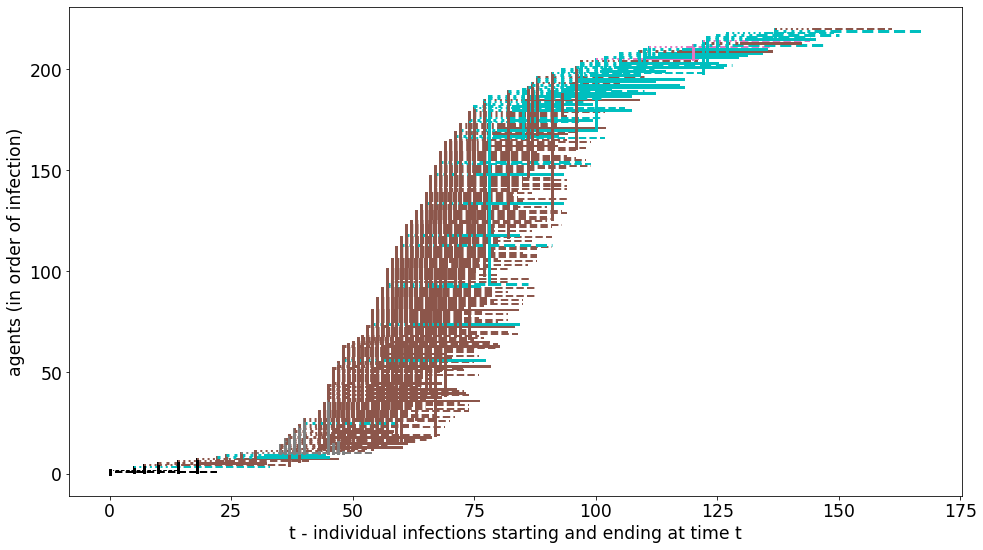
\includegraphics[scale=0.2]{withShort1.png}             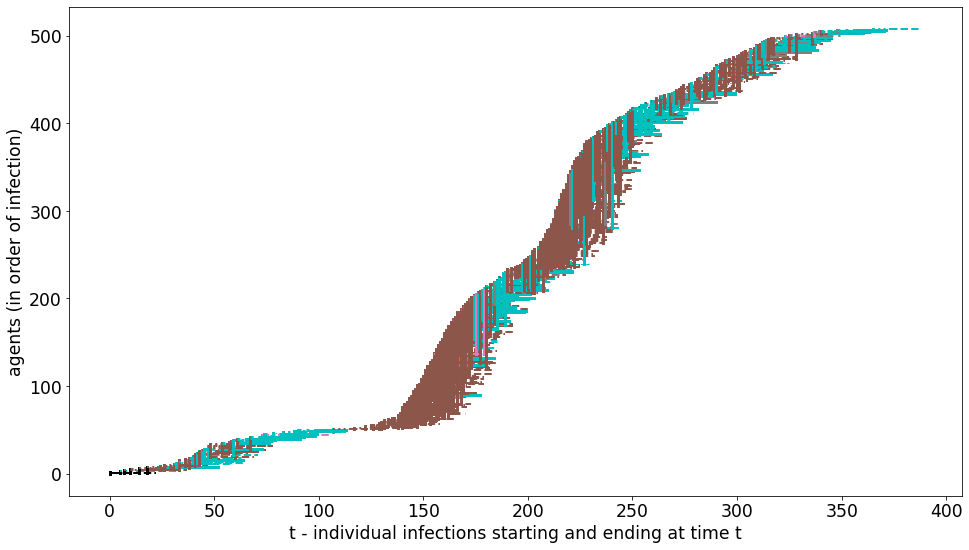
\includegraphics[scale=0.2]{withShort1A.png} 
%\hspace{0.2cm}
\center
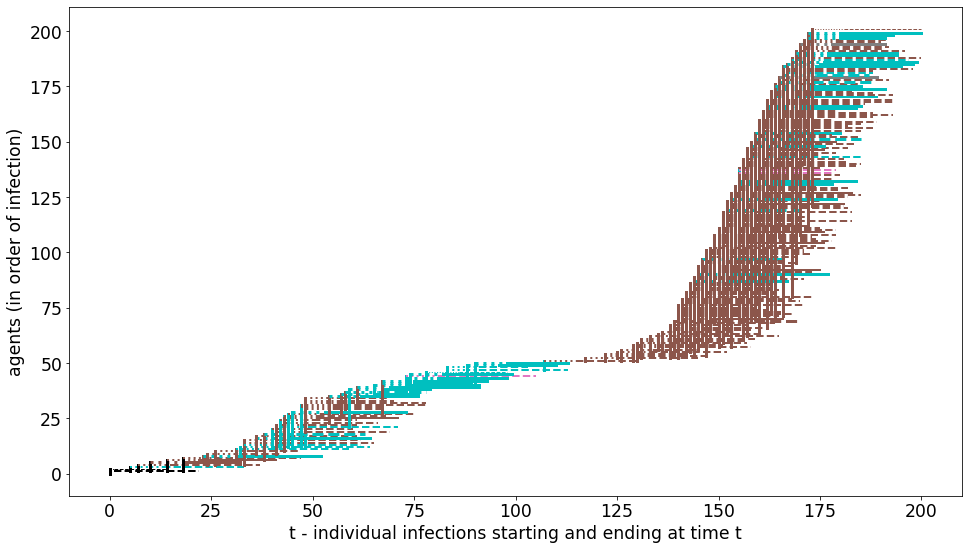
\includegraphics[scale=0.2]{withShort1A200.png}     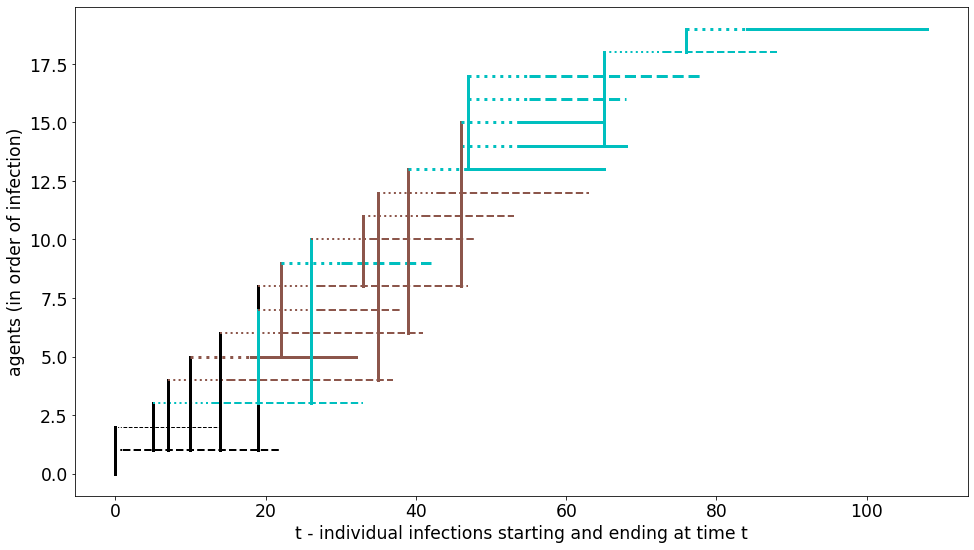
\includegraphics[scale=0.2]{withShort1B.png} \\
\caption{(\emph{top left}) an epidemic with containment measures, showing a highly significant effect of workplaces (brown);
 (\emph{top right}) the effects of stopping fragile workers at day 20, with a positive result, but home contagions (cyan) keep alive the pandemic, exploding again in workplaces (brown); (\emph{bottom left}) the same analyzing the first 200 infections with evidence of the event around day 110 with the new phase due to a unique asymptomatic worker, and (\emph{bottom right}) stopping fragile workers and any case of fragility at day 15, also isolating nursing homes} 
\label{fourSequences}
\end{figure}

\begin{comment}
withShort1.png         %using SIsaR 9.4.2 as is (basic control) with 123456_22314, file ex123456_22313.csv;
withShort1A.png      %using SIsaR 9.4.2 as is (basic control + 20 sFW 1,i.e., stop Fragile Workers) with 123456_22314, file ex123456_22314A.csv;
withShort1A200.png %using SIsaR 9.4.2 as is (basic control + 20 sFW 1,i.e., stop Fragile Workers) with 123456_22314, file ex123456_22314A.csv;
withShort1B.png       %using SIsaR 9.4.2 as is (basic control + $$$) with 123456_22314, file ex123456_22314B.csv;
\end{comment}

The four pictures, related to epidemics starting precisely in the same way, represent an evolving narrative, that:

\begin{enumerate}

\item starts from the observation of an epidemic in which workplaces have an evident role in sustaining the spreading of the virus, despite the adoption of the non-pharmaceutical containment measures adopted locally and at the national level;

\item adopts a counterfactual limitation holding back fragile workers from factories (any workplace), with some initial success, but with a \emph{bridge} to a phase 2;

\item\label{micromicro} deepens the situation of the specific agent operating as a bridge, a regular (non-fragile) worker infected at work by another regular worker infected at home by a fragile agent;

\item introduces a more substantial  control, anticipating at Feb \nth{15} the limitation to fragile workers and stopping the mobility of all fragile people from Feb \nth{20} with evident positive effect, having the whole epidemic very few contagions and lasting a limited number of days.

\end{enumerate}

In our model, the fragile workers are those 55 years old or more; in this scheme, if they cannot work remotely from home, they are supposed to obtain regular sick pay (see Sections \ref{CBanalysis} and \ref{c8} for considerations).

This kind of analysis is a source of suggestions for interventions, also if we cannot validate them only with micro studies, as in bullet point \ref{micromicro} above. 

Summarizing: 

\begin{itemize}
\setlength{\itemsep}{0pt}
\item we confirm the interest of the knowledge that we can extract from contagion sequences; 
\item we suggest, as an integrative example, the simulation of Fig. \ref{6b}  in Appendix \ref{appContagion}, showing many cases of fragile workers diffusing the infection;
\item finally, we will use a more systematic data exploration, in Section \ref{app1000run}, as summarized in Section \ref{keyResultsS}.
\end{itemize}


\section{Simulation repetition and emerging key results}
\label{keyResultsS}

Following the trace of Fig. \ref{fourSequences}, we now explore systematically the introduction of factual, counterfactual, and prospective interventions to control the spread of the contagions. Each simulation run---whose length coincides with the disappearance of symptomatic or asymptomatic contagion cases---is a datum in a wide scenario of variability in time and effects. Consequently, we need to represent compactly the results emerging from batches of repetitions, to compare each batch's basic assumption's consequences.

We adopted blocks of one thousand repetitions (or more, for other analyses not reported here). Besides summarizing the results with the usual statistical indicators, we adopted the technique of the heat-maps (see Appendix \ref{app1000run}). 

In this way, we endorse the \cite{steinmann2020don} incitement.
\begin{quote}
We urge those attempting to model COVID-19 for decision support to acknowledge the deep uncertainties surrounding the pandemic, and to employ Decision Making under Deep Uncertainty methods such as exploratory modelling, global sensitivity analysis, and robust decision-making in their analysis to account for these uncertainties.
\end{quote}


Using the calculations of Appendix \ref{app1000run}, we build the Table \ref{keyResultsT}, starting from a zero interventions case (no controls of any type) e moving toward actions more and more specific (always non-pharmaceutical). In the table, we report four indicators: the total number of symptomatic subjects in nursing homes; the total number of symptomatic subjects; the total number of symptomatic-asymptomatic-deceased subjects; the duration of the epidemic. The scale to which refer the data is the Piedmont population, i.e., 4,350 million people. We report the mean and standard deviation of each measure in the batch of 1,000 repetitions of the simulated epidemic. In the last column, we write the section of the appendix, reporting the results of the specific batch calculation.



\begin{table}[H]
\center
\footnotesize
%\small
\begin{tabular}{lrrrrr}
\toprule
Scenarios                       & total sym.          &  total sym.  & total sym.       & days~~~~ & Section \\
{}                                     & in nursing         &                    & asympt.~~~   \\
{}                                     & homes~~~~~    &                    & deceased~~  \\
\midrule
1.~no control                       &       4.65~         &  851.12~     &  2253.48         &  340.10~   &  \ref{EpidemicsWithoutControlS} \\
                                        &       (7.89)         &  (288.52)    &  (767.58)         &  (110.21) \\
\midrule
2.~basic controls, no         &        4.51~         &   158.55~    &  416.98~         &  196.97~   & \ref{EpidemicsWithAndNoSchoolS} \\
 school in Sep 2020       &       (7.39)         &   (174.10)     &  (462.94)        &  (131.18) \\
\midrule
3.~basic controls, schools   &       4.24~        &  153.71~    &      409.73~       &  199.35~   & \ref{EpidemicsWithAndSchoolS} \\
 open in Sep 2020           &       (7.29)        &  (168.55)   &     (454.12)        &  (129.00) \\
\midrule
4.~basic controls, stop        &      4.32~         &  120.17~   &      334.68~         &  181.10~     & \ref{EpidemicsFWsS} \\
 fragile workers, no          &      (7.48)         &   (149.10)  &     (413.90)         &   (125.46) \\
 schools in Sep 2020   \\
\midrule
5.~basic controls, nur-          &       3.41~      &  150.53~     &     408.08~         &  201.76~     & \ref{EpidemicsNHsS} \\
 sing homes isol., no         &       (6.88)     &   (172.48)    &     (467.54)         &  (138.15) \\
 schools in Sep 2020   \\
\midrule
6.~basic controls, stop          &       4.38~      &   154.15~    &     408.50~         &  195.81~     & \ref{EpidemicsFragileS} \\
 fragile people, no            &       (7.52)      &   (170.22)    &      (456.08)        &  (129.52) \\
 schools in Sep 2020   \\
\midrule
7.~basic controls, stop f.       &       3.25~      &   105.63~    &     302.62~          &  174.39~     & \ref{EpidemicsNoAllFragileS} \\
 workers \&  f. people \&   &       (6.60)      &   (134.80)   &     (382.14)          &  (121.82) \\
 n. h. isol., no sch, Sep.        \\
 \midrule
8.~b. controls, stop f. workers  &     3.46~     &  124.10~    &    397.05~           &  200.31~     & \ref{EpidemicsNoAllFragileFacsOnS} \\
 \&  f. people \& nur. h. isol.,  &  (6.65)       &  (132.42)   &    (399.64)           &  (121.46) \\
 \& factories op., no sch. Sep. \\
\midrule
9.~b. controls, stop f. workers  &     3.63~     &  116.55~   &    374.68~           &  195.28~     & \ref{EpidemicsNoAllFragileFacsOnSchOnS} \\
 \&  f. people \& nur. h. isol.,  &   (6.96)      &  (130.91) &     (394.66)           &  (119.33) \\
 \& factories op., sch. open Sep. \\
\bottomrule
\end{tabular}

\caption{Report of the key results, with mean and (std)}
\label{keyResultsT}
\end{table}

The values of the standard deviations are impressive, as a signal of the difficulties in forecasting an epidemic. Those estimates are primarily due to very different durations of the virus diffusion, being this occurrence also linked to thin events like that in bullet point \ref{micromicro} in Section  \ref{seqSuggPol}. That event is not on scale to the population size (1:1000), but it is a single agent acting, as observed in reality, in many situations.

General notes: data refer to a population of 4,350 subjects (1:1,000 of Piedmont people). We over-represent nursing homes to have visibility of the phenomenon, both as the spatial distribution of these institutions and each unit dimension. As we clarify in the supporting information (see note \ref{modOnLine}), in scale, we would have less than one nursing home, with 30 hosts; we created five with a total value of around 60 hosts.

A comment to Table \ref{keyResultsT}, following the different blocks, row by row:

\begin{enumerate}
\setlength{\itemsep}{0pt}

\item\label{cf1} we start with a counterfactual analysis with 1,000 runs of the epidemic model without any non-pharmaceutical containment measures; The results are extraordinary heavy, both as symptomatic persons (19.6\% of the population) and total infected  people (51.8\%); the mean duration of the epidemics is close to one year;

\item\label{f1}  the second step, factual, is that of introducing the sequence of non-pharmaceutical containment measures of Appendix \ref{appCalendar}, again in a batch of 1,000 runs; we have now 3,6\% and 9,6\% rates, with a diminution highly relevant, and a mean duration half of the preceding one; if you look at the heat-maps in Sections \ref{EpidemicsWithoutControlS} and \ref{EpidemicsWithAndNoSchoolS}, where we classify the results in terms of durations and infections of each epidemic in the double histograms, you can see that the difference is astonishing; a note: the actual Piedmont, where the curve of the symptomatic cases flattened with the end of May, with around 30 thousand subjects, is included in the cell in the first row, immediately to the right of the mode in Fig. \ref{EpidemicsWithAndNoSchoolHM}, considering that here we have to triplicate the number symptomatic subject to have the total measure of infected agents;

\item\label{f2} in this prospective analysis, we have the same sequence of containment measures of the previous case, with the difference that from September \nth{14} (2020) schools are open; the rates on infection are a bit lower than those of case 2, the duration is very close; certainly standard deviation signal a relevant variability, but similar to the previous one; the rates of infection decrease, here and also in the similar step from case 8 to 9, with a possible interpretation: keeping in school the students for a part of the day decreases contagions in other regularly frequented spaces, where they could find more contagious people;

\item\label{cf2} the fourth case is again a counterfactual one, always with the regular containment measures (and schools closed in September), but supposing that we had followed the strategy of Section \ref{seqSuggPol}, not admitting the fragile employees in the workplaces, from February \nth{20}; the positive effect is evident, with the infection rates now at 2.8\% and 7.7\%;

\item\label{cf3} we decided to investigate separately two other counterfactual possibilities, always with the regular containment measures (and schools closed in September), starting with the isolation of the nursing homes, forbidding visits, separating the operators, and creating a buffer zone prohibiting to everyone to get close to nursing homes, again from February \nth{20}; we have some positive effect, but limited; sure, a bit more relevant for the nursing homes, where the residual infections are coming from contagions occurred before the blocking decision;


\item\label{cf4} the second separate counterfactual verification, in the same conditions of the previous trial, is that of keeping all fragile people in isolation at home but, as in reality occurred, the workers can continue to move to go to their workplaces; the benefits are again quite limited;

\item\label{cf5} with the \nth{7} batch of simulated epidemics, we put in action all the measures of the counterfactual experiments number \ref{cf2}, \ref{cf3}, and \ref{cf4}; the results, in this case, are highly positive with the infection rates about symptomatic people and total ones reduced to 2.4\% and 7.0\%, with the minimal mean duration in the table; as a synthesis, we are preserving all fragile people;

\item\label{cf6} continuing in the counterfactual perspective, we verify the consequence of not closing factories and workplaces of any kind; we measure some worsening if we compare these rates with the previous ones, but they are always a lot better than those of the factual case \ref{f1};

\item\label{cf7} finally, as the last step, we add the decision of opening the schools in September, again---as for case \ref{f2}---with some improvement if compared with the same situation with the schools closed.

\end{enumerate}

To summarize, the actions carried out were of extraordinary effect and usefulness. Still, it would have been possible to add other forms of action that could have had lower overall costs. Therefore, measures to preserve the situation at risk for all fragile people and at the same time to not stop the economy and society indiscriminately.



\section{Cost-benefit analysis of the of interventions}
\label{CBanalysis}

Considering  the different interventions of Table \ref{keyResultsT} we can evaluate \ldots

First of all, the costs for the attribution of sick pay to workers who are compulsorily absent from work, if they are not able to carry out telework activities and the benefits of continuing economic activities \ldots

Internal contents in Sections \ref{seqSuggPol}. 
\ref{keyResultsS} with Table \ref{keyResultsT}, \ref{c7}, 
\ref{EpidemicsFWsS}, 
\ref{EpidemicsNoAllFragileS}.

An interesting reference is \cite{doi:10.1111/ijcp.13674}, where \ldots WORKS IN PROGRESS.

WORKS IN PROGRESS.


\section{Summarizing}

WORKS IN PROGRESS.

For future works:
\begin{itemize}

\item add: transportation; discotheques; movement regulation by hours; \ldots;

\item use \url{https://terna.github.io/SLAPP/};

\item refer to \url{https://www.quantamagazine.org/how-to-assess-risks-during-the-coronavirus-pandemic-20200925/?utm_source=phplist1469&utm_medium} as a source of the parameters and to \url{https://www.gleamproject.org} for data and analysis.

\end{itemize}

\section*{Acknowledgements}

Many thanks to Simone Landini, Nizar Mansour, Fabio Pammolli, Enrico Scalas, and Federico Tedeschi for precious discussions, insights, and critics. The usual disclaimer applies.

\appendix

\section{Appendix: Analyzing examples of contagion sequences}
\label{appContagion}

We introduce nine cases, mainly as examples. For technical details, look at Appendix \ref{appHowItWorks}. Among those cases, we have the set of sequences commented in Section \ref{seqSuggPol}, which are a special source of suggestions for policies. Still, other suggestions can emerge by observing the other sequences reported here or that can be generated. Each run of the program produces a different sequence that can be analyzed, as explained in the Appendix, using the program at \url{https://github.com/terna/contagionSequence}.

Notice that, with containment measures, sometimes the sequences get thinner, involving few agents. 
Then, they can start again or---with a bit of luck---stop. A typical situation is that of Fig. \ref{0} where, on day 43, we have a unique spreading agent (that became infected in a nursing home, so orange). The agent continues the infection, with two further contagions (looking into the simulation run's details, this agent is a nursing home operator). Without the containment measures, the flow of the contagions is ample, excluding the situation of Figs. \ref{4a} and \ref{4b} where, in the beginning, the epidemic seems not to start.

The agents starting the infection correspond to the two black segments in each picture's bottom left corner. They are  \emph{coming from nowhere}, as external events. The evolution of each simulation is strongly influenced by randomness, as in reality: the New York Times of March \nth{5}, 2020, offered us since the beginning, a non-conventional analysis on <<The Covid-19 Riddle: Why Does the Virus Wallop Some Places and Spare Others?>>\footnote{\url{https://www.nytimes.com/2020/05/03/world/asia/coronavirus-spread-where-why.html }.}. The title of the last paragraph is <<Roll of the Dice>> and starts with:

\begin{quote}
Finally, most experts agree that there may be no single reason for some countries to be hit and others missed. The answer is likely to be some combination of the above factors, as well as one other mentioned by researchers: sheer luck.

Countries with the same culture and climate could have vastly different outcomes if one infected person attends a crowded social occasion, turning it into what researchers call a super-spreader event.
\end{quote}

\subsubsection{How to analyze the figures of this section}
\label{howToAnalyze}

How the figures of this appendix work: refer as an example to Fig. \ref{2}, related to a simulation of a very short duration. We have a few infected people there, so the graphical representation is detailed without the need to enlarge the picture, which is always possible if you use the article's pdf file.

We start with two externally infected people, represented by the two black segments in the picture's bottom-left corner. The segments' length means each subject's infection period; these are asymptomatic (dashed lines, refer to Appendix \ref{appHowItWorks}). The first one is a regular agent (as the thickness suggests). The second one is a robust agent; by convention, we introduce them in the simulation at the end of the incubation period. The first agent transmits (follow the vertical link) the contagion to another regular agent in a workplace (brown color); the second is not producing contagions. The third agent, asymptomatic after the incubation period (dotted line), infects four agents: three in the workplace (two of them fragile, as we see from the thickness of the line), and the last one (a fragile person) at home (cyan). The sequence continues until the \nth{24} agent, infected in a hospital, infecting no one in turn.

We have to remember that we work here on a scale of 1:1000. Still, in interpreting these sequences, it is worth considering the agent to agent transmission as examples of events related to single persons.

\subsection{Epidemics without containment measures}

The cases of Sections \ref{c1}, \ref{c2}, and \ref {c3} report simulation without any kind of non-pharmaceutical measures.


\subsubsection{Case 1: workplaces, nursing homes, and homes}
\label{c1}

The epidemic in Fig. \ref{3a} lasted about 350 days and affected about 2,500 people on a total of 4,350(in the 1:1,000 scale). In the beginning, the leading presence is that of contagions in nursing homes (orange) and in workplaces (brown), but successively a significant role is that of the contagions at home (cyan); some effect is coming from hospitals. We can better understand the starting sequence in Fig. \ref{3b}, where we report only the first 200 contagion cases.
  
\begin{comment}

this is a memo on the order of sources, explaining numbers

                           using SIsaR 9.4.2 as is (basic control) with 123456_22313
withShort0.png   ex123456_22313.csv
withShort1.png   ex123456_22314.csv
withShort2.png   ex123456_22315.csv

                           using SIsaR 9.4.2 (basic control + 20 sFW 1,i.e., stop Fragile Workers)  with 123456_22314
withShort1A.png ex123456_22314A.csv
withShort1A200.png 

                           using SIsaR 9.4.2 (basic control + $$$)  with 123456_22314                           
 								$$$
								15 sFW 1     NB at 15
								15 limlock 1
								15 %PeopleAny 0  NB stop fragile at 15
								15 %PeopleNot 90
								15 PvNH 0   NB at 15 stop visist
								28 %PeopleNot 80
withShort1B.png ex123456_22314B.csv

          		 from 'SIsaR_0.9.4.1tmp experiments 2 seeds no control-table_5000.csv'
no3a.png	        	 noControl_10932215_10933923.csv
no3b.png
no4a.png           noControl_12518034_12520144.csv
no4b.png
no5a.png           noControl_13790741_13792228.csv
no5b.png

                          from 'SIsaR_0.9.4.1 experiments 2 seeds with control-table_10000.csv'
with6a.png        withControl_268411_270578.csv
with6b.png
with7a.png        withControl_2722110_2723664.csv
with7b.png
with8a.png        withControl_473323_474697.csv
with8b.png

\end{comment}



\begin{figure}[H]
\begin{center}
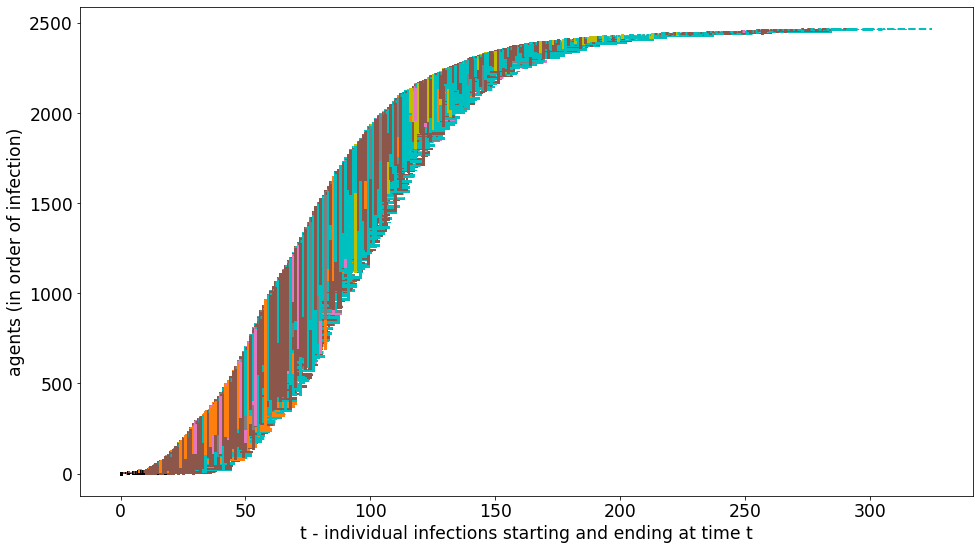
\includegraphics[width=0.7\textwidth]{no3a.png} % no control case 10932215 10933923 in SIsaR_0.9.4.1tmp experiments 2 seeds no control-table_5000.csv, file noControl_10932215_10933923.csv
\caption{Case 1, without containment measures: contagions in nursing homes (orange), workplaces (brown), homes (cyan), hospitals (pink)}
\label{3a}
\end{center}
\end{figure}

\begin{figure}[H]
\begin{center}
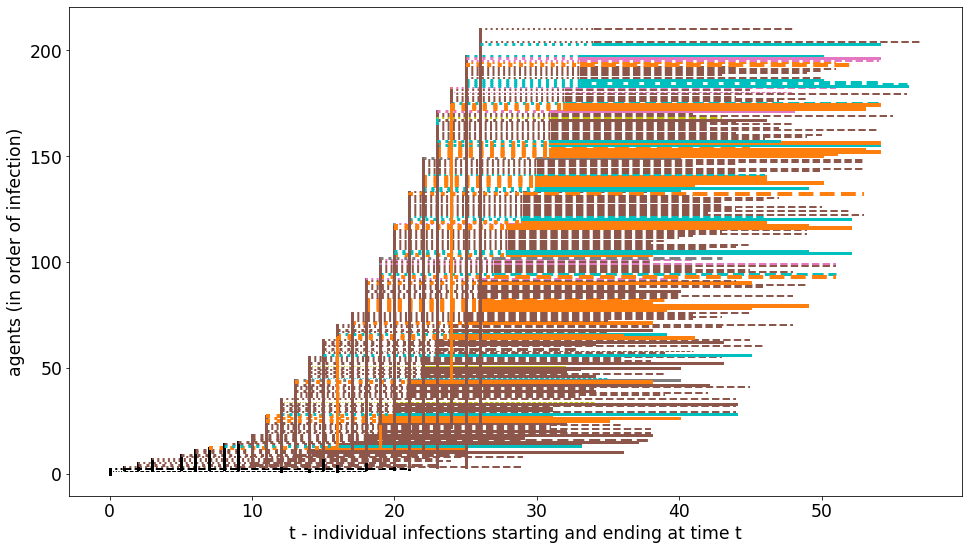
\includegraphics[width=0.7\textwidth]{no3b.png} % no control case 10932215_10933923 in SIsaR_0.9.4.1tmp experiments 2 seeds no control-table_5000.csv, file noControl_10932215_10933923.csv
\caption{Case 1, without containment measures, first 200 infections with the main contribution of nursing homes (orange) and workplaces (brown)}
\label{3b}
\end{center}
\end{figure}

\subsubsection{Case 2: multiple sources of infection}
\label{c2}

In Fig.~\ref{4a}, we have another history of contagion without control---always with everything open, including schools---with the epidemic that alternates contagions at home (cyan), in hospitals (pink). in the workplaces (brown), with a decisive initial role of nursing homes (orange), as shown in Fig. \ref{4b}, which enlarges the first 200 cases. There is also a bit of school contribution, but very limited. Around day 70, a unique contagion at home has the role of having the epidemic continuing.

\begin{figure}[H]
\begin{center}
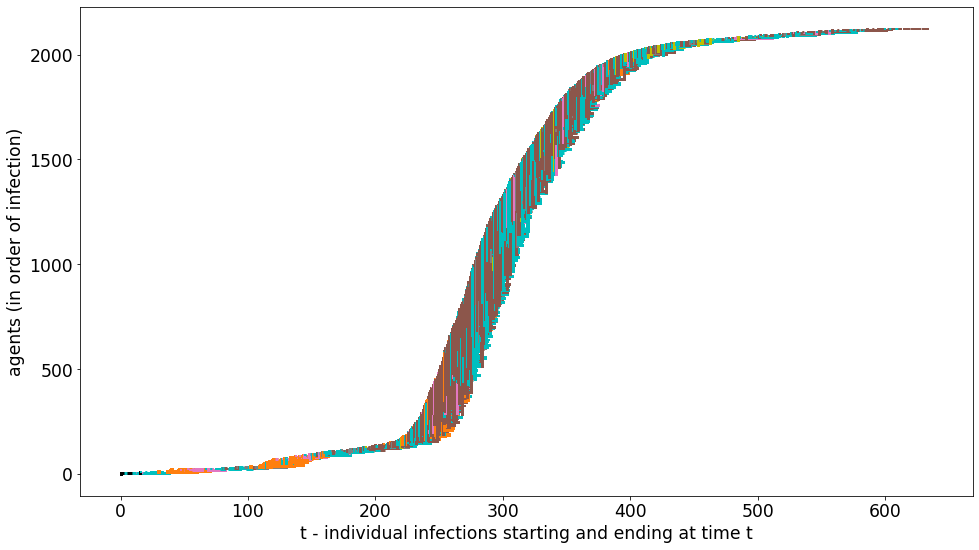
\includegraphics[width=0.7\textwidth]{no4a.png}% no control case 12518034 12520144 in SIsaR_0.9.4.1tmp experiments 2 seeds no control-table_5000.csv, file noControl_12518034_12520144.csv

\caption{Case 2, without containment measures: nursing homes (orange) as starter}
\label{4a}
\end{center}
\end{figure}

\begin{figure}[H]
\begin{center}
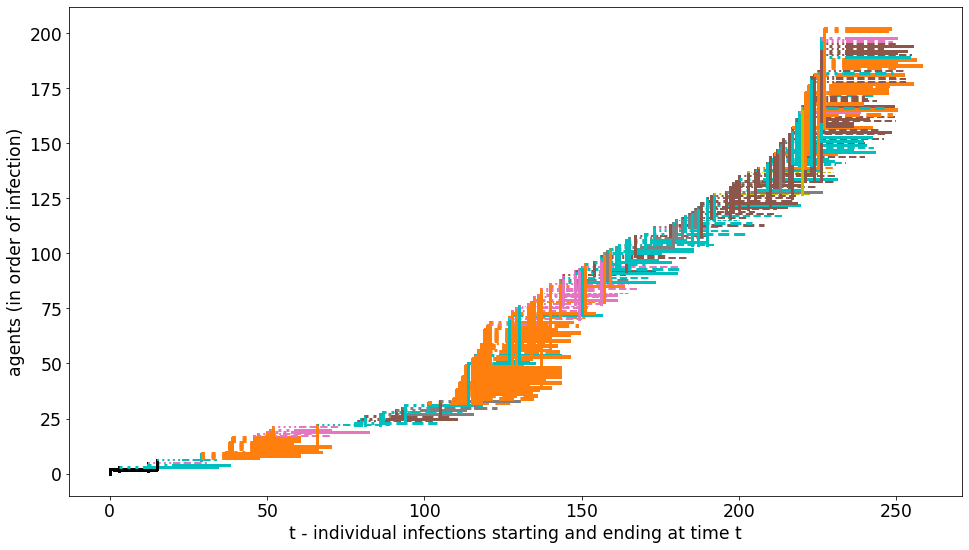
\includegraphics[width=0.7\textwidth]{no4b.png}% no control case 12518034 12520144 in SIsaR_0.9.4.1tmp experiments 2 seeds no control-table_5000.csv, filee noControl_12518034_12520144.csv

\caption{Case 2, without containment measures, first 200 infections: nursing homes (orange) as starter and around day 70 a unique contagion at home continuing the epidemic}
\label{4b}
\end{center}
\end{figure}

\subsubsection{Case 3: workplaces and homes}
\label{c3}

Without containment measures: an initial deep effect of contagions is in workplaces and at home, both in Fig. \ref{5a} and very clearly in Fig. \ref{5b}, where workplace and home effects are interleaving. Analyzing the dimension and the style (solid or dashed, as in Section \ref{lineStyle}) of the segments representing the agents infected in the early phase, we observe\footnote{To better observe, it is possible to enlarge the picture in the pdf version of the article.} the role of fragile agents, also asymptomatic (dashed segments).



\begin{figure}[H]
\begin{center}
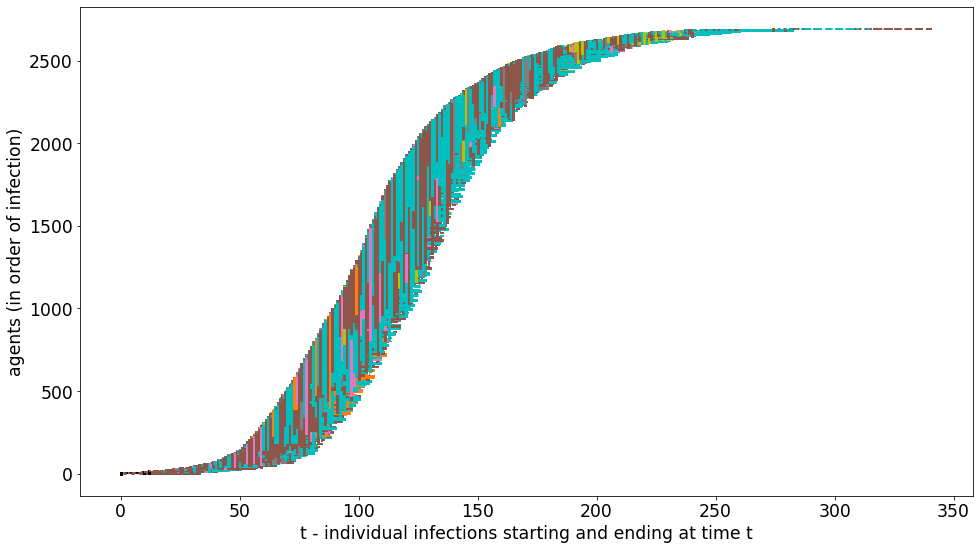
\includegraphics[width=0.7\textwidth]{no5a.png}% no control case 113790741 13792228 in SIsaR_0.9.4.1tmp experiments 2 seeds no control-table_5000.csv, file noControl_13790741 13792228.csv
\caption{Case 3, without containment measures: an initial deep effect of contagions in workplaces (brown) and homes (cyan)}
\label{5a}
\end{center}
\end{figure}

\begin{figure}[H]
\begin{center}
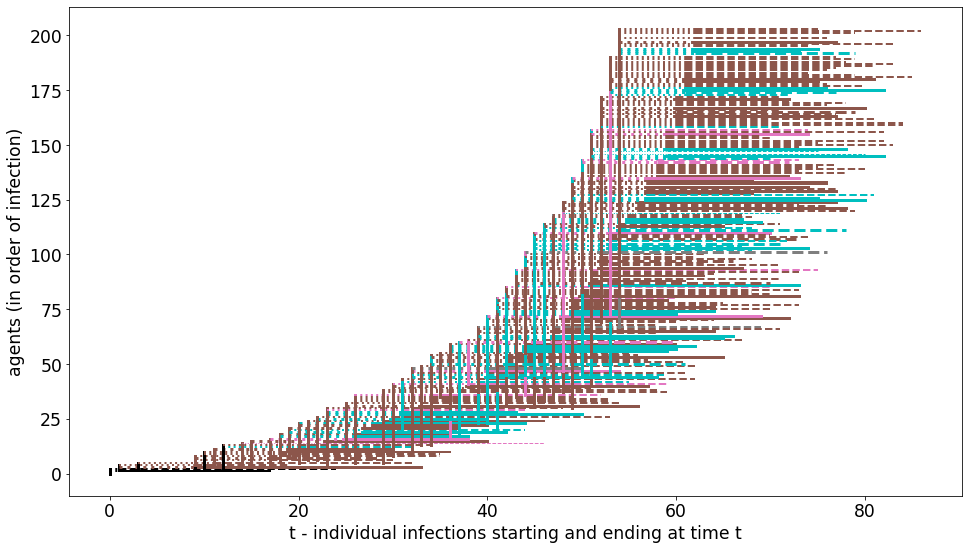
\includegraphics[width=0.7\textwidth]{no5b.png}% no control case 113790741 13792228 in SIsaR_0.9.4.1tmp experiments 2 seeds no control-table_5000.csv, file noControl_13790741 13792228.csv
\caption{Case 3, without containment measures, first 200 infections: the initial deep effect of contagions in workplaces (brown) and homes is due in the initial steps to fragile persons, also asymptomatic}
\label{5b}
\end{center}
\end{figure}

\subsection{Cases with containment measures}

The cases of Sections \ref{c4}, \ref{c5}, and \ref {c6} report simulation incorporating the non-pharmaceutical measures of the calendar in Appendix \ref{AppCalendar}.

\subsubsection{Case 4, again the importance of workplaces (brown) and homes (cyan)}
\label{c4}

We adopt here the non-pharmaceutical measures of the calendar in Appendix \ref{appCalendar}. The school is always close also in September. 
In Figs. \ref{6a} and \ref{6b}, we again can verify the importance of the workplaces and homes in diffusing the infection, with the critical signal, in Fig. \ref{6b}, of many cases of fragile workers diffusing the disease.


\begin{figure}[H]
\begin{center}
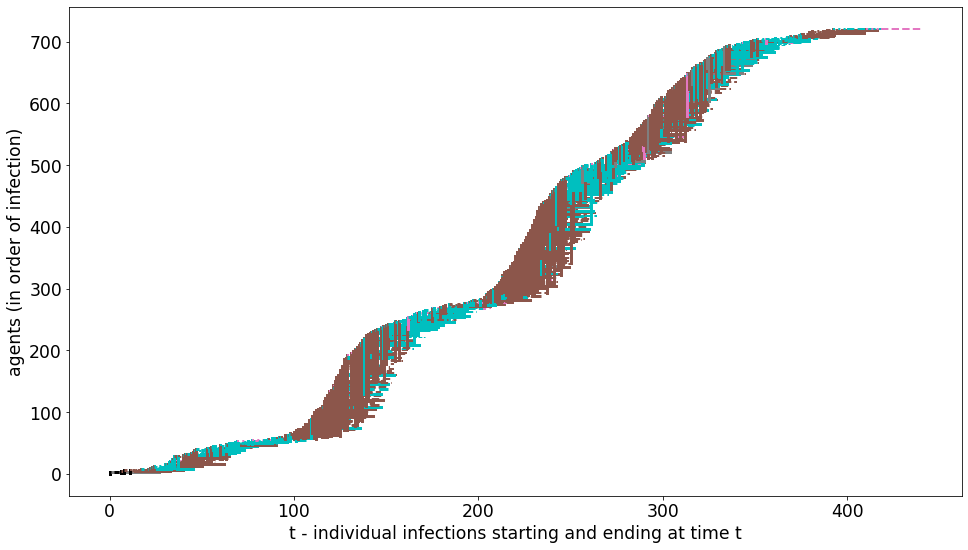
\includegraphics[width=0.7\textwidth]{with6a.png}% with control case 268411 270578 in SIsaR_0.9.4.1 experiments 2 seeds with control-table_10000.csv, file withControl_268411_270578.csv
\caption{Case 4, with containment measures: another case of strong contribution of workplaces (brown) and homes (cyan) to epidemic diffusion}
\label{6a}
\end{center}
\end{figure}

\begin{figure}[H]
\begin{center}
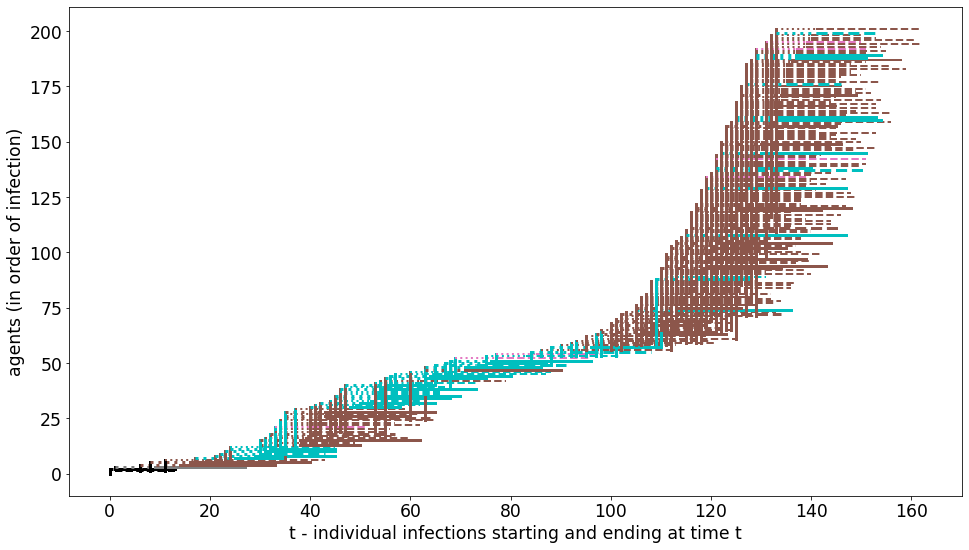
\includegraphics[width=0.7\textwidth]{with6b.png}% with control case 268411 270578 in SIsaR_0.9.4.1 experiments 2 seeds with control-table_10000.csv, file withControl_268411_270578.csv
\caption{Case 4, with containment measures, first 200 infections: after day 100 we observe many significant cases of fragile workers diffusing the infection}
\label{6b}
\end{center}
\end{figure}

\subsubsection{Case 5, with workplaces (brown), hospitals (pink), nursing homes (orange) and homes (cyan), then workplaces (brown)}
\label{c5}

In this case, we have a sequence of highly interlaced different contagion places.

\begin{figure}[H]
\begin{center}
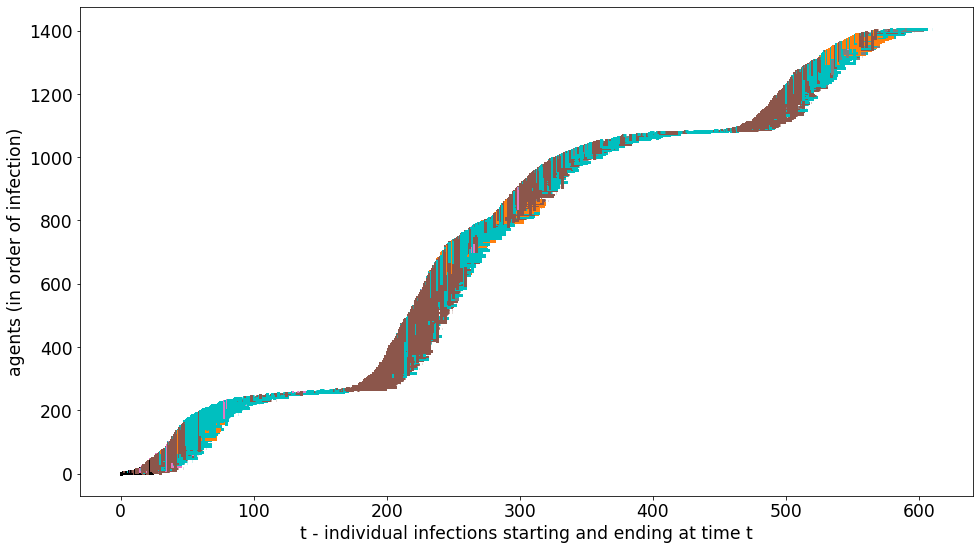
\includegraphics[width=0.7\textwidth]{with7a.png}% with control case 2722110 2723664 in SIsaR_0.9.4.1 experiments 2 seeds with control-table_10000.csv, file withControl_2722110_2723664.csv
\caption{Case 5, with containment measures: workplaces (brown), hospitals (pink), nursing homes (orange) and homes (cyan), then workplaces}
\label{7a}
\end{center}
\end{figure}

\begin{figure}[H]
\begin{center}
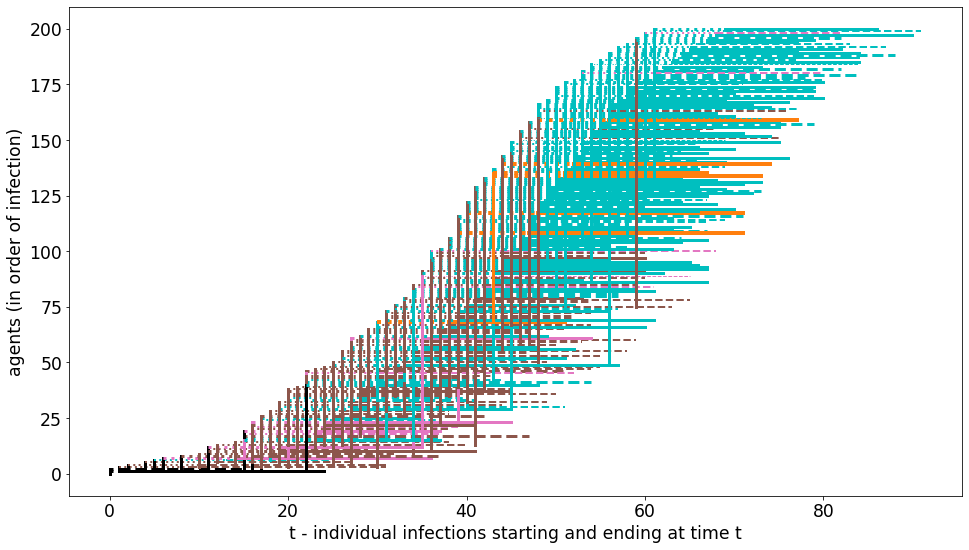
\includegraphics[width=0.7\textwidth]{with7b.png}% with control case 2722110 2723664 in SIsaR_0.9.4.1 experiments 2 seeds with control-table_10000.csv, file withControl_2722110_2723664.csv
\caption{Case 5, with containment measures, first 200 infections: in the beginning workplaces (brown), hospitals (pink), nursing homes (orange) and homes (cyan) interweaving}
\label{7b}
\end{center}
\end{figure}

\subsubsection{Case 6, with workplaces (brown) and nursing homes (orange)}
\label{c6}


In this case, nursing homes' initial role is evident, with a large number of extra-fragile people infected as symptomatic. Looking at the vertical links, we see in Fig. \ref{8b} them frequently coming from fragile or extra-fragile people (the last ones, infected in a nursing home, so orange).

\begin{figure}[H]
\begin{center}
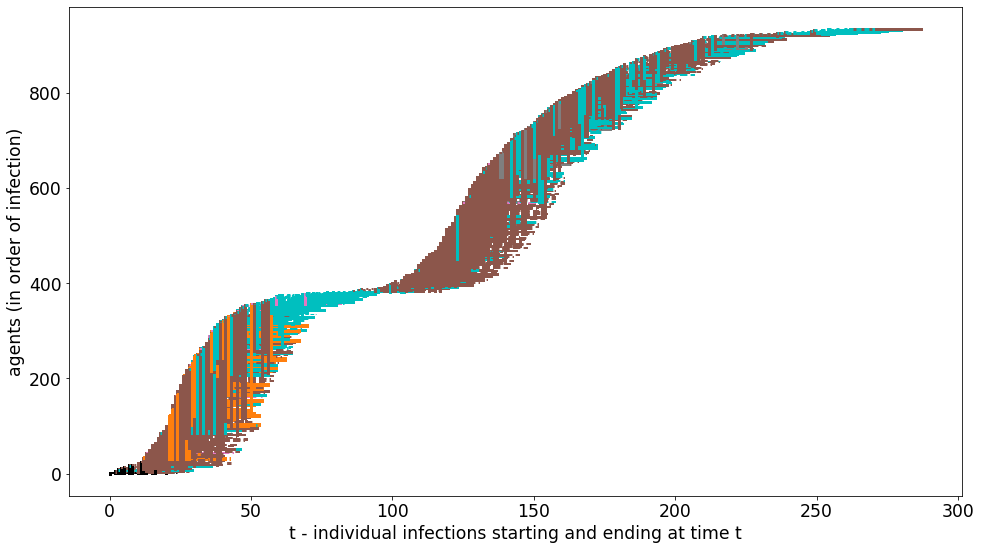
\includegraphics[width=0.7\textwidth]{with8a.png}% with control case 473323 474697 in SIsaR_0.9.4.1 experiments 2 seeds with control-table_10000.csv, file withControl_473323_474697.csv
\caption{Case 6, with containment measures: workplaces (brown), nursing homes (orange), homes (cyan)}
\label{8a}
\end{center}
\end{figure}

\begin{figure}[H]
\begin{center}
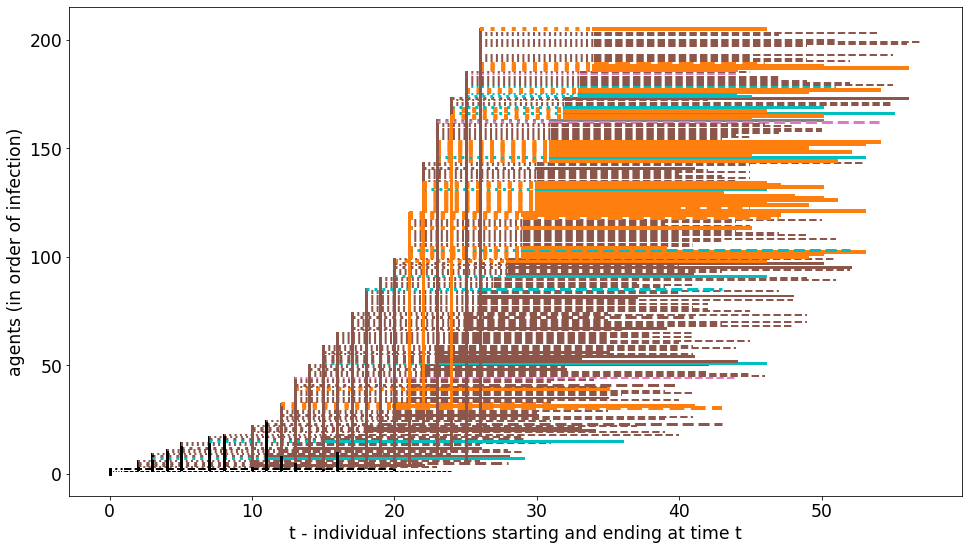
\includegraphics[width=0.7\textwidth]{with8b.png}% with control case 473323 474697 in SIsaR_0.9.4.1 experiments 2 seeds with control-table_10000.csv, file withControl_473323_474697.csv
\caption{Case 6, with containment measures, first 200 infections: workplaces (brown) and nursing homes (orange) strictly interweaving}
\label{8b}
\end{center}
\end{figure}

\subsection{Short running epidemic, with containment measures}

The cases of Sections \ref{c7}, \ref{c8}, and \ref {c9} report simulation with short duration, incorporating the non-pharmaceutical measures of the calendar in Appendix \ref{appCalendar}.


\subsubsection{Case 7, only nursing homes (orange)}
\label{c7}


In Fig. \ref{0} we have an extreme epidemic situation, involving uniquely the nursing homes.

\begin{figure}[H]
\begin{center}
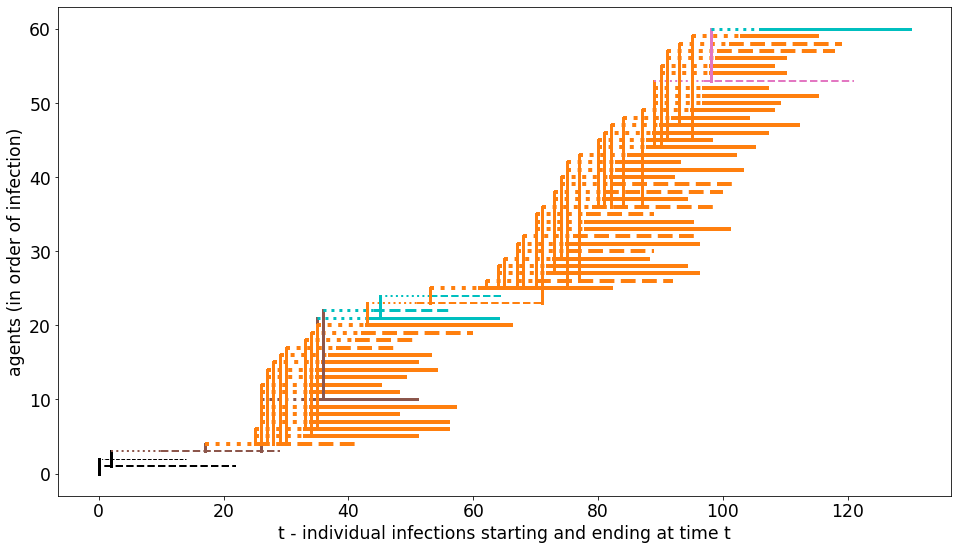
\includegraphics[width=0.7\textwidth]{withShort0.png}%using SIsaR 9.4.2 as is (basic control) with 123456_22313, file ex123456_22313.csv
\caption{Case 7, with containment measures: the effect of nursing homes (orange)}
\label{0}
\end{center}
\end{figure}


\subsubsection{Case 8 with workers and control of fragility in two steps}
\label{c8}


The analysis of the sequences of contagion in this appendix makes evident the relevance of fragility, in workplaces and nursing homes, to sustain the diffusion of the SARS-CoV-2 virus. It suggests the importance of considering together two different views: that of the defense of the health of every single person, especially if fragile, and that of the protection of collective health.

The document 
<<Economic Aspects of the COVID-19 Crisis in the UK>>\footnote{\url{https://rs-delve.github.io/reports/2020/08/14/economic-aspects-of-the-covid19-crisis-in-the-uk.html}.}
of the DELVE initiative\footnote{DELVE---Data Evaluation and Learning for Viral Epidemics---is a multi-disciplinary group, convened by the Royal Society, to support a data-driven approach to learning from the different approaches countries are taking to managing the covid-19 pandemic. \url{https://rs-delve.github.io}.}
dedicates special attention to work conditions in virus spreading and the problems related to workers' preventive or immediate isolation, both fragile or with early mild symptoms.

\begin{quote}
Current sick pay arrangements create a financial disincentive to self-isolate, with half of workers continuing to work through mild coronavirus symptoms, which in turn makes it more difficult to control transmission. Reviewing statutory sick pay could help incentivise those with symptoms to self-isolate.

(\ldots)

Low-earning workers are also in jobs that tend to be harder to perform remotely, increasing their risk of unemployment or infection in the workplace, if mitigating steps are not taken.
\end{quote}

The proposal here is to devote maximum preventive attention to fragile workers, leaving them home with sick pays (in reality, a part of the would work remotely from home). This situation is different from limiting fragile people's movements because it is mainly related to ages more advanced than those of the workers. Besides, that kind of decision allows people to move to go to the workplace. 

Intervention policies must properly design this non-pharmaceutical contention measure, defining the sick pay and the related rules with modalities and levels adequate to avoid the problems quoted above.

\begin{figure}[H]
\begin{center}
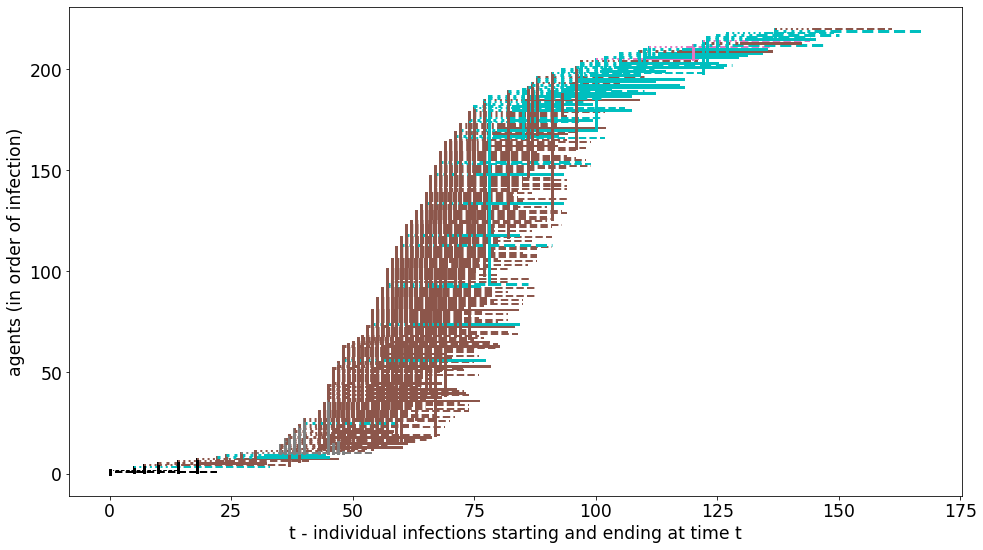
\includegraphics[width=0.7\textwidth]{withShort1.png}%using SIsaR 9.4.2 as is (basic control) with 123456_22314
\caption{Case 8, with containment measures: a highly significant effect of workplaces (brown)}
\label{1}
\end{center}
\end{figure}


In Fig. \ref{1} we have the first of the four pictures already seen in Section \ref{seqSuggPol}. It is a case in which the workplace's effect as an elective area of contagion is powerful. The epidemic lasts around 170 days. We introduce a further containment measure to the regular ones (those of Appendix \ref{appCalendar}). From the \nth{20} day of the simulated period, fragile workers are no more participating in work activity (into our simulated Piedmont, they correspond to a quota of around the 5\% of the whole population). The effect, in Fig. \ref{1A} is very positive in stopping the initial workplace action, but a series of home contagions restarts the epidemic, again in workplaces. As we see in Fig. \ref{1B}, here we have the effect of an unlucky circumstance: that of a unique agent, infected at home, again spreading the infection in the workplaces. We show this event to confirm the high variability in epidemic developments. Considering batches of 1,000 simulations, as in Section \ref{EpidemicsFWsS}, the positive effect of the proposed measure is well evident.

\begin{figure}[H]
\begin{center}
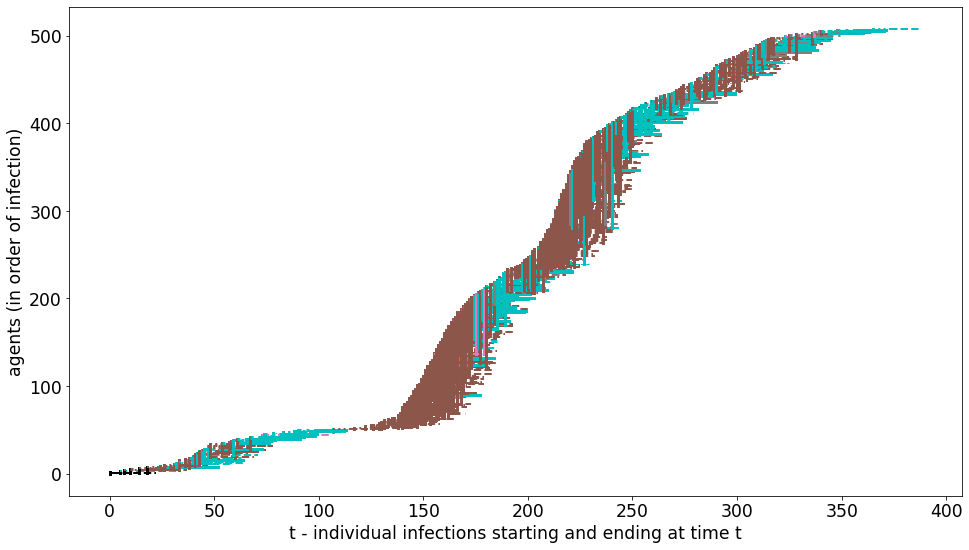
\includegraphics[width=0.7\textwidth]{withShort1A.png}%using SIsaR 9.4.2 as is (basic control + 20 sFW 1,i.e., stop Fragile Workers) with 123456_22314
\caption{Case 8, with containment measures, stopping fragile workers at day 20, with a positive result, but home contagions (cyan) keep alive the pandemic, which explodes again in workplaces (brown)}
\label{1A}
\end{center}
\end{figure}

\begin{figure}[H]
\begin{center}
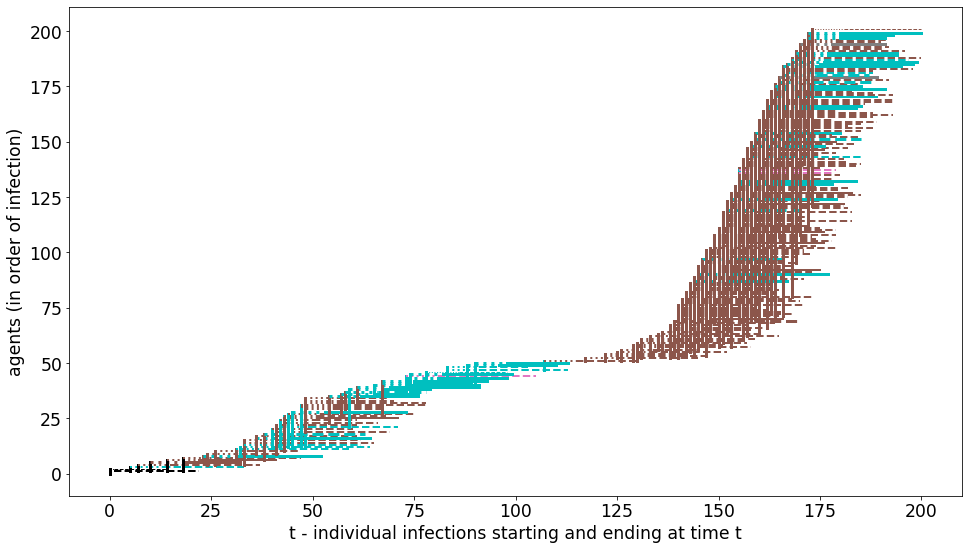
\includegraphics[width=0.7\textwidth]{withShort1A200.png}%using SIsaR 9.4.2 as is (basic control + 20 sFW 1,i.e., stop Fragile Workers) with 123456_22314
\caption{Case 8, with containment measures, stopping fragile workers at day 20, with a positive effect, but home contagions (cyan) keep alive the pandemic, which explodes again in workplaces (brown), first 200 infections with evidence of the event around day 110 with the new phase due to a unique asymptomatic worker}
\label{1A200}
\end{center}
\end{figure}

As a most substantial measure, we try a general stop of any fragility since the \nth{15} day of the simulated period. The positive effect is evident in Fig. \ref{1B}, with a short-lasting epidemics, affecting few people. A note: in the batch analysis of Appendix \ref{app1000run}, we always use the \nth{20} day as a turning point.

\begin{figure}[H]
\begin{center}
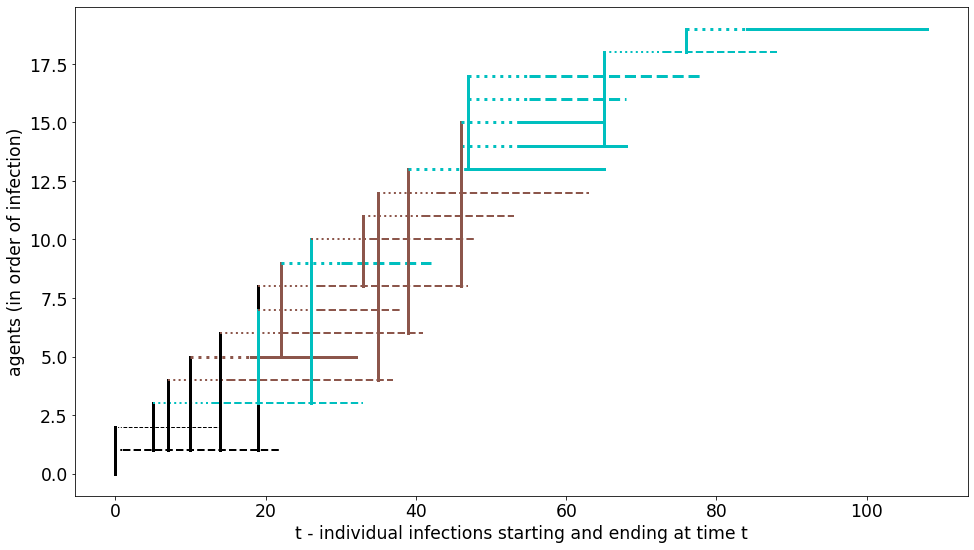
\includegraphics[width=0.7\textwidth]{withShort1B.png}%using SIsaR 9.4.2 as is (basic control + $$$) with 123456_22314
\caption{Case 8, with containment measures, stopping fragile workers and any case of fragility at day 15, also isolating nursing homes}
\label{1B}
\end{center}
\end{figure}



\subsubsection{Case 9, a spontaneously stopping epidemic}
\label{c9}

To finish this series of examples, in Fig. \ref{2} we show the case of an epidemic spontaneously stopping quickly, using the regular non-pharmaceutical containment measures.

\begin{figure}[H]
\begin{center}
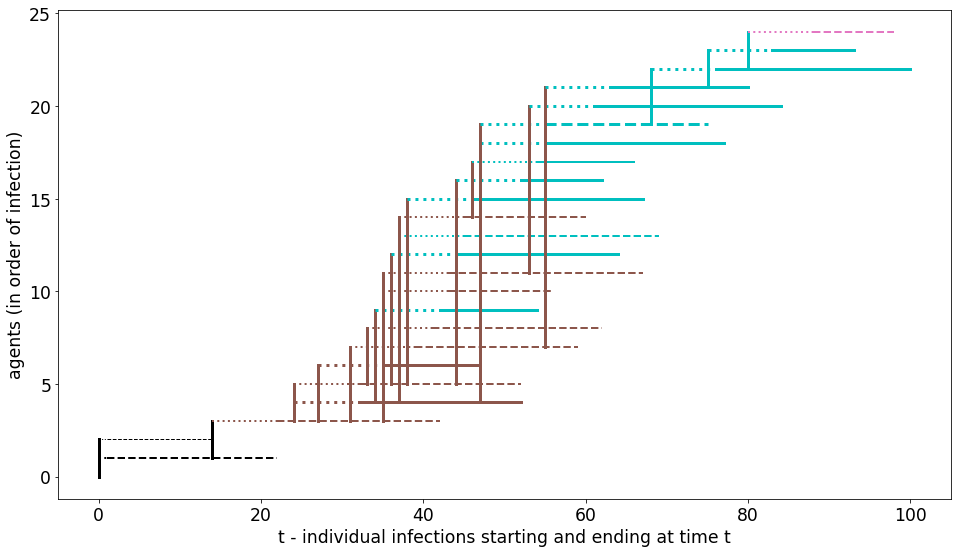
\includegraphics[width=0.7\textwidth]{withShort2.png}%using SIsaR 9.4.2 as is (basic control) with 123456_22315, file ex123456_22315.csv
\caption{Case 9, with containment measures: a spontaneously stopping epidemic in  short period}
\label{2}
\end{center}
\end{figure}



\section{Appendix: batches of 1,000 simulated experiments generating data for policy proposals}
\label{app1000run}

To systematically explore the results of the different simulations, taking into account the variability of the outcomes, we produce batches of 1,000 runs via the tool \verb|BehaviorSpace| of NetLogo. \verb|BehaviorSpace| creates \verb|csv| files that we analyze with the programs at 
\url{https://github.com/terna/readSIsaR_BatchResults}. The different titles correspond to those of this appendix; it is also possible to run the codes directly from there.

We report here the results of the calculations, both as descriptive statistics and as heat-maps. A heat-map is a double histogram; in our application, it displays each simulated epidemic's duration in the $x$ axis and the count of the symptomatic, asymptomatic, and deceased agents in the $y$ axis. The cells contain the number of cases. The data are always on a scale 1:1000.

The descriptive statistics are about: the total number of symptomatic subjects in nursing homes, the total number of symptomatic subjects, the total number of symptomatic-asymptomatic-deceased subjects, the duration of the epidemic.

\subsection{Epidemics without containment measures}
\label{EpidemicsWithoutControlS}

Here we are without any control, and the school always open. The values of Table \ref{EpidemicsWithoutControlT} are scary, and the concentration of the cases in the heat-map of Fig. \ref{EpidemicsWithoutControlHM} shows that, except a few instances spontaneously concluding in a short period (left bottom corner), we have a heavy \emph{cloud}\footnote{In the 2020 Summer, in the mountain, one of the authors saw the cloud configuration reporte at \url{https://terna.to.it/simul/HeatmapInTheCloud.png}; a curious coincidence.} of cases lasting one year or one year and a half, hitting (as symptomatic, asymptomatic and deceased) from 2.400 to 3,200 people on a total of 4,350.

The calculations of this Section are reported synthetically in Section \ref{keyResultsS} and in the related Table \ref{keyResultsT}.

\begin{table}[H]
\center
\small
\begin{tabular}{lrrrr}
\toprule
{} & total sym.        &  total sym. & total sym.     & days~~~~ \\
{} & in nursing        &                  & asympt.~~~  & \\
{} & homes~~~~~  &                  & deceased~~ & \\
\midrule
count &     962.00 &             1000.00 &                 1000.00 & 1000.00 \\
mean  &       4.65 &              851.12 &                 2253.48 &  340.10 \\
std   &       7.89 &              288.52 &                  767.58 &  110.21 \\
min   &       0.00 &                0.00 &                    2.00 &   12.00 \\
25\%   &       0.00 &              849.00 &                 2246.75 &  317.00 \\
50\%   &       0.00 &              924.00 &                 2442.00 &  357.00 \\
75\%   &       8.00 &              998.00 &                 2639.25 &  399.25 \\
max   &      54.00 &             1240.00 &                 3592.00 &  638.00 \\
\bottomrule
\end{tabular}

\label{EpidemicsWithoutControlT}
\caption{Epidemics without containment measures}
\end{table}

\begin{figure}[H]
\begin{center}
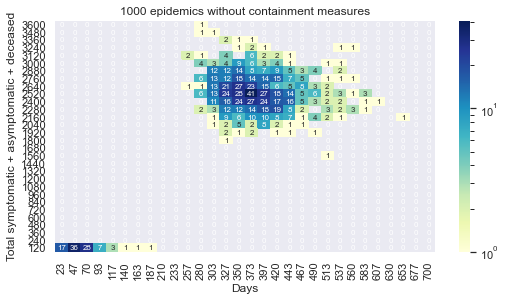
\includegraphics[width=0.7\textwidth]{HM30_readRunResults1k_noControl_plusHMlog.png}
\caption{Epidemics without containment measures (logarithmic scale for colors)}
\label{EpidemicsWithoutControlHM}
\end{center}
\end{figure}

\subsection{Epidemics with basic non-pharmaceutical containment measures, no school in September 2020}
\label{EpidemicsWithAndNoSchoolS}

We follow here the calendar of controls of Appendix \ref{appCalendar}. Comparing the values of Table \ref{EpidemicsWithAndNoSchoolT} with those of Table \ref{EpidemicsWithoutControlT} we measure a strong difference. The content of Fig. \ref{EpidemicsWithAndNoSchoolT} shows the variability of results; most of all, a completely different distribution of the events if compared with Fig. \ref{EpidemicsWithAndNoSchoolT}. School is always closed in this simulation.

As in Section \ref{keyResultsS} we have here the possibility referring to actual Piedmont, where the curve of the symptomatic cases flattened with the end of May, with around 30 thousand subjects; with that datum, the region is included in the cell in the first row, immediately to the right of the mode in Fig. \ref{EpidemicsWithAndNoSchoolHM}, considering that here we have to triplicate the number symptomatic subject to obtain the full measure of infected agents.


\begin{table}[H]
\center
\small
\begin{tabular}{lrrrr}
\toprule
{} & total sym.        &  total sym. & total sym.     & days~~~~ \\
{} & in nursing        &                  & asympt.~~~  & \\
{} & homes~~~~~  &                  & deceased~~ & \\
\midrule
count &     946.00 &             1000.00 &                 1000.00 & 1000.00 \\
mean  &       4.51 &              158.55 &                  416.98 &  196.97 \\
std   &       7.39 &              174.10 &                  462.94 &  131.18 \\
min   &       0.00 &                0.00 &                    2.00 &   12.00 \\
25\%   &       0.00 &                9.75 &                   20.00 &   89.75 \\
50\%   &       0.00 &               82.00 &                  219.00 &  154.00 \\
75\%   &       8.00 &              287.00 &                  778.75 &  298.00 \\
max   &      46.00 &              749.00 &                 1916.00 &  611.00 \\
\bottomrule
\end{tabular}

\label{EpidemicsWithAndNoSchoolT}
\caption{Epidemics with basic non-pharmaceutical containment measures, no school in September 2020}
\end{table}


\begin{figure}[H]
\begin{center}
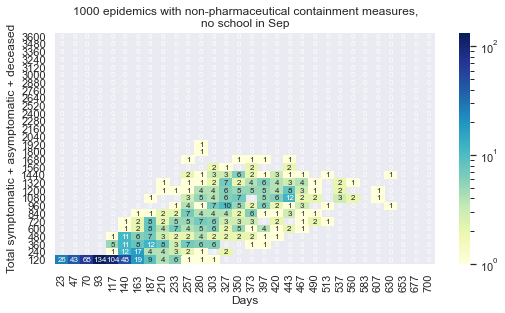
\includegraphics[width=0.7\textwidth]{HM30_readRunResults1k_withControl_plusHMlog.png}
\caption{Epidemics with basic non-pharmaceutical containment measures, no school in September 2020 (logarithmic scale for colors)}
\label{EpidemicsWithAndNoSchoolHM}
\end{center}
\end{figure}




\subsection{Epidemics with basic non-pharmaceutical containment measures, school open in September 2020}
\label{EpidemicsWithAndSchoolS}


What if the school would be open in September? We note some reduction of the infections in Table \ref{EpidemicsWithAndSchoolT}, maybe because concentrating the student in schools for a part of the day, we have fewer people around. The same observation holds for Section \ref{EpidemicsNoAllFragileFacsOnSchOnS}.

\begin{table}[H]
\center
\small
\begin{tabular}{lrrrr}
\toprule
{} & total sym.        &  total sym. & total sym.     & days~~~~ \\
{} & in nursing        &                  & asympt.~~~  & \\
{} & homes~~~~~  &                  & deceased~~ & \\
\midrule
count &     946.00 &             1000.00 &                 1000.00 & 1000.00 \\
mean  &       4.24 &              153.71 &                  409.73 &  199.35 \\
std   &       7.29 &              168.55 &                  454.12 &  129.00 \\
min   &       0.00 &                0.00 &                    2.00 &   13.00 \\
25\%   &       0.00 &                9.00 &                   18.75 &   95.00 \\
50\%   &       0.00 &               81.50 &                  231.50 &  154.00 \\
75\%   &       6.00 &              269.50 &                  770.00 &  309.25 \\
max   &      42.00 &              738.00 &                 1907.00 &  617.00 \\
\bottomrule
\end{tabular}

\label{EpidemicsWithAndSchoolT}
\caption{Epidemics with basic non-pharmaceutical containment measures, schools open in September 2020}
\end{table}


\begin{figure}[H]
\begin{center}
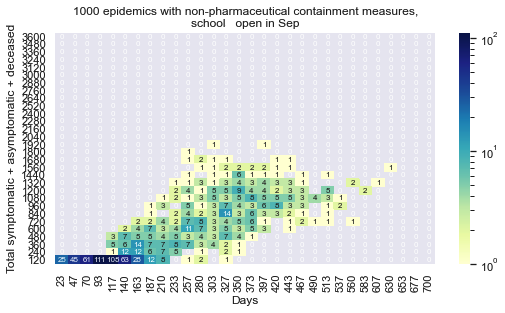
\includegraphics[width=0.7\textwidth]{HM30_readRunResults1k_basicControl_schoolOpenSept_plusHMlog.png}
\caption{Epidemics with basic non-pharmaceutical containment measures, schools open in September 2020 (logarithmic scale for colors)}
\label{EpidemicsWithAndSchoolHM}
\end{center}
\end{figure}



\subsection{Epidemics with immediate stop of fragile workers, non-pharmaceutical containment measures, no school in September 2020}
\label{EpidemicsFWsS}


In Table \ref{EpidemicsFWsT} and in Fig. \ref{EpidemicsFWsHM} we verify with a batch of 1,000 runs the analysis of Sections \ref{seqSuggPol} and \ref{c7}. The verification of the strategy of stopping fragile workers with the epidemic early warnings, here at February \nth{20}, gives a significant reduction of the infected people and the simulation duration. Anticipating the stop on February \nth{15}, only some limited advantages are emerging.

\begin{table}[H]
\center
\small
\begin{tabular}{lrrrr}
\toprule
{} & total sym.        &  total sym. & total sym.     & days~~~~ \\
{} & in nursing        &                  & asympt.~~~  & \\
{} & homes~~~~~  &                  & deceased~~ & \\
\midrule
count &     955.00 &             1000.00 &                 1000.00 & 1000.00 \\
mean  &       4.32 &              120.17 &                  334.68 &  181.10 \\
std   &       7.48 &              149.10 &                  413.90 &  125.46 \\
min   &       0.00 &                0.00 &                    2.00 &   13.00 \\
25\%   &       0.00 &                8.00 &                   17.00 &   86.00 \\
50\%   &       0.00 &               41.00 &                   94.00 &  136.00 \\
75\%   &       6.00 &              210.00 &                  586.25 &  267.25 \\
max   &      44.00 &              745.00 &                 2043.00 &  746.00 \\
\bottomrule
\end{tabular}

\label{EpidemicsFWsT}
\caption{Epidemics with the immediate stop of fragile workers, non-pharmaceutical containment measures, no school in September 2020}
\end{table}


\begin{figure}[H]
\begin{center}
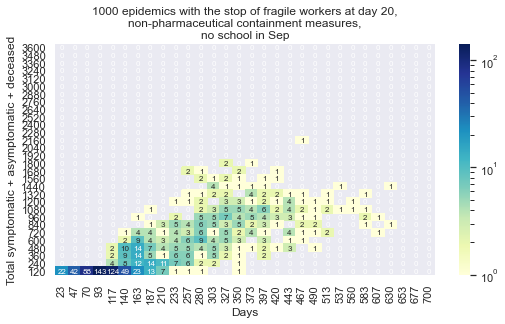
\includegraphics[width=0.8\textwidth]{HM30_readRunResults1k_with_sFW_at20_plusHMlog.png}
\caption{Epidemics with the immediate stop of fragile workers, non-pharmaceutical containment measures, no school in September 2020 (logarithmic scale for colors)}
\label{EpidemicsFWsHM}
\end{center}
\end{figure}

\subsection{Epidemics with absolute isolation of nursing homes, non-pharmaceutical containment measures, no school in September 2020}
\label{EpidemicsNHsS}

As explained in Section \ref{keyResultsS} commenting the Table \ref{keyResultsT}, some strategies are separately explored. If considered separately, each one gives positive but limited results. 

First trial: we put in action the prohibition of the visits to the nursing homes and the isolation of the related operators, plus creating a buffer zone segregating nursing homes and hospitals. No school in September.

\begin{table}[H]
\center
\small
\begin{tabular}{lrrrr}
\toprule
{} & total sym.        &  total sym. & total sym.     & days~~~~ \\
{} & in nursing        &                  & asympt.~~~  & \\
{} & homes~~~~~  &                  & deceased~~ & \\
\midrule
count &     955.00 &             1000.00 &                 1000.00 & 1000.00 \\
mean  &       3.41 &              150.53 &                  408.08 &  201.76 \\
std   &       6.88 &              172.48 &                  467.54 &  138.15 \\
min   &       0.00 &                0.00 &                    2.00 &   12.00 \\
25\%   &       0.00 &                8.00 &                   18.00 &   89.00 \\
50\%   &       0.00 &               70.00 &                  196.00 &  147.50 \\
75\%   &       0.00 &              268.25 &                  756.50 &  312.25 \\
max   &      47.00 &              737.00 &                 1977.00 &  695.00 \\
\bottomrule
\end{tabular}

\label{EpidemicsNHsT}
\caption{Epidemics with the absolute isolation of nursing homes, non-pharmaceutical containment measures, no school in September 2020}
\end{table}


\begin{figure}[H]
\begin{center}
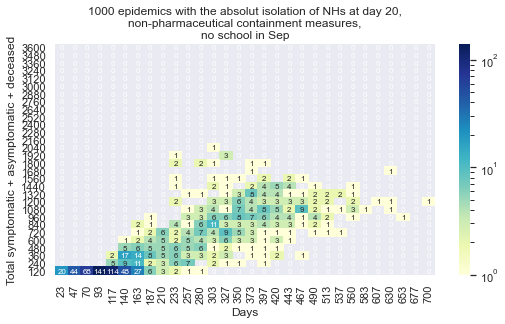
\includegraphics[width=0.8\textwidth]{HM30_readRunResults1k_with_NH_OP_BZ_at20_plusHMlog.png}
\caption{Epidemics with the absolute isolation of nursing homes, non-pharmaceutical containment measures, no school in September 2020 (logarithmic scale for colors)}
\label{EpidemicsNHsHM}
\end{center}
\end{figure}


\subsection{Epidemics stopping fragile people, non-pharmaceutical containment measures, no school in September 2020}
\label{EpidemicsFragileS}


Second trial: we lock fragile people at home, but the fragile workers continue their activity?no school in September..

\begin{table}[H]
\center
\small
\begin{tabular}{lrrrr}
\toprule
{} & total sym.        &  total sym. & total sym.     & days~~~~ \\
{} & in nursing        &                  & asympt.~~~  & \\
{} & homes~~~~~  &                  & deceased~~ & \\
\midrule
count &     952.00 &             1000.00 &                 1000.00 & 1000.00 \\
mean  &       4.38 &              154.15 &                  408.50 &  195.81 \\
std   &       7.52 &              170.22 &                  456.08 &  129.52 \\
min   &       0.00 &                0.00 &                    2.00 &   14.00 \\
25\%   &       0.00 &                9.00 &                   19.00 &   90.00 \\
50\%   &       0.00 &               93.50 &                  251.00 &  154.50 \\
75\%   &       7.25 &              264.25 &                  747.50 &  294.00 \\
max   &      57.00 &              820.00 &                 2079.00 &  660.00 \\
\bottomrule
\end{tabular}

\label{EpidemicsFragileT}
\caption{Epidemics limiting fragile people mobility, non-pharmaceutical containment measures, no school in September 2020}
\end{table}


\begin{figure}[H]
\begin{center}
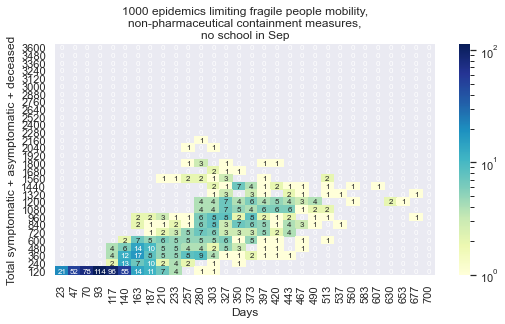
\includegraphics[width=0.8\textwidth]{HM30_readRunResults1k_with_Frag_at20_plusHMlog.png}
\caption{Epidemics limiting fragile people mobility, non-pharmaceutical containment measures, no school in September 2020 (logarithmic scale for colors)}
\label{EpidemicsFragileHM}
\end{center}
\end{figure}


\subsection{Epidemics excluding fragility of any type, non-pharmaceutical containment measures, no school in September 2020}
\label{EpidemicsNoAllFragileS}

We put in action together all the limitations of Sections \ref{EpidemicsFWsS}, \ref{EpidemicsNHsS}, and \ref{EpidemicsFragileS}. The school is closed in September. The reduction of the infected people and of the duration, in Table \ref{EpidemicsNoAllFragileT} and in Fig. \ref{EpidemicsNoAllFragileHM}, are relevant, representing the best result obtained.


\begin{table}[H]
\center
\small
\begin{tabular}{lrrrr}
\toprule
{} & total sym.        &  total sym. & total sym.     & days~~~~ \\
{} & in nursing        &                  & asympt.~~~  & \\
{} & homes~~~~~  &                  & deceased~~ & \\
\midrule
count &     947.00 &             1000.00 &                 1000.00 & 1000.00 \\
mean  &       3.25 &              105.63 &                  302.62 &  174.39 \\
std   &       6.60 &              134.80 &                  382.14 &  121.82 \\
min   &       0.00 &                0.00 &                    2.00 &   12.00 \\
25\%   &       0.00 &                8.00 &                   17.00 &   84.75 \\
50\%   &       0.00 &               37.50 &                   84.00 &  131.00 \\
75\%   &       0.00 &              173.00 &                  515.50 &  252.25 \\
max   &      40.00 &              728.00 &                 1844.00 &  651.00 \\
\bottomrule
\end{tabular}

\label{EpidemicsNoAllFragileT}
\caption{Epidemics excluding fragility of any type, non-pharmaceutical containment measures, no school in September 2020}
\end{table}


\begin{figure}[H]
\begin{center}
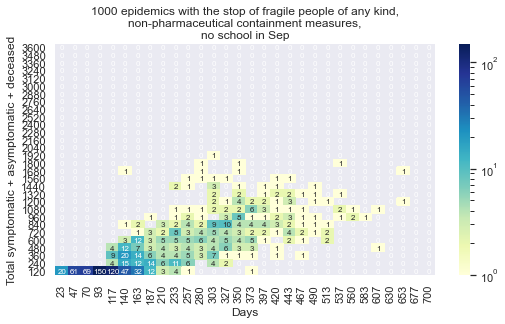
\includegraphics[width=0.8\textwidth]{HM30_readRunResults1k_with_NoAllFrag_at20_plusHMlog.png}
\caption{Epidemics excluding fragility of any type, non-pharmaceutical containment measures, no school in September 2020 (logarithmic scale for colors)}
\label{EpidemicsNoAllFragileHM}
\end{center}
\end{figure}



\subsection{Epidemics excluding fragility of any type, non-pharmaceutical containment measures, factories open, no school in September 2020}
\label{EpidemicsNoAllFragileFacsOnS}

We confirm the setting of Section \ref{EpidemicsNoAllFragileS}, but now with the factories (shops, offices, etc.) always open. The results are acceptable.

\begin{table}[H]
\center
\small
\begin{tabular}{lrrrr}
\toprule
{} & total sym.        &  total sym. & total sym.     & days~~~~ \\
{} & in nursing        &                  & asympt.~~~  & \\
{} & homes~~~~~  &                  & deceased~~ & \\
\midrule
count &     960.00 &             1000.00 &                 1000.00 & 1000.00 \\
mean  &       3.46 &              124.10 &                  397.05 &  200.31 \\
std   &       6.65 &              132.42 &                  399.64 &  121.46 \\
min   &       0.00 &                0.00 &                    2.00 &   14.00 \\
25\%   &       0.00 &                9.00 &                   19.00 &   95.75 \\
50\%   &       0.00 &               85.00 &                  279.00 &  188.00 \\
75\%   &       5.00 &              202.25 &                  707.00 &  284.00 \\
max   &      41.00 &              868.00 &                 2140.00 &  714.00 \\
\bottomrule
\end{tabular}

\label{EpidemicsNoAllFragileFacsOnT}
\caption{Epidemics excluding fragility of any tyoe, non-pharmaceutical containment measures, with factories open, no school in September 2020}
\end{table}


\begin{figure}[H]
\begin{center}
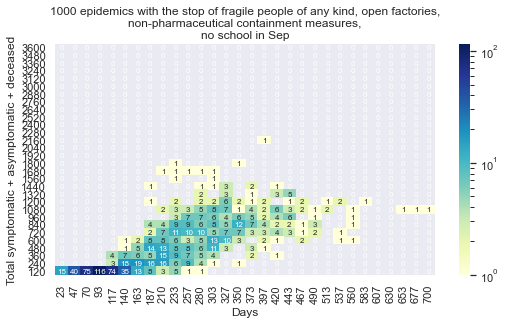
\includegraphics[width=0.8\textwidth]{HM30_readRunResults1k_with_NoAllFrag_openFacs_at20_plusHMlog.png}
\caption{Epidemics excluding fragility of any type, non-pharmaceutical containment measures, with factories open, no school in September 2020 (logarithmic scale for colors)}
\label{EpidemicsNoAllFragileFacsOnHM}
\end{center}
\end{figure}




\subsection{Epidemics excluding fragility of any type, non-pharmaceutical containment measures, factories open, schools open in September 2020}
\label{EpidemicsNoAllFragileFacsOnSchOnS}

Finally, to the setting of Section \ref{EpidemicsNoAllFragileFacsOnS}, we add the decision of opening the schools in September. The results are acceptable, with a slight improvement, already noticed in Section \ref{EpidemicsWithAndSchoolS}.

\begin{table}[H]
\center
\small
\begin{tabular}{lrrrr}
\toprule
{} & total sym.        &  total sym. & total sym.     & days~~~~ \\
{} & in nursing        &                  & asympt.~~~  & \\
{} & homes~~~~~  &                  & deceased~~ & \\
\midrule
count &     949.00 &             1000.00 &                 1000.00 & 1000.00 \\
mean  &       3.63 &              116.55 &                  374.68 &  195.28 \\
std   &       6.96 &              130.91 &                  394.66 &  119.33 \\
min   &       0.00 &                0.00 &                    2.00 &   12.00 \\
25\%   &       0.00 &                9.00 &                   20.00 &   91.00 \\
50\%   &       0.00 &               68.00 &                  225.00 &  180.50 \\
75\%   &       5.00 &              186.00 &                  651.50 &  275.25 \\
max   &      45.00 &              665.00 &                 1844.00 &  666.00 \\
\bottomrule
\end{tabular}

\label{EpidemicsNoAllFragileFacsOnSchOnT}
\caption{Epidemics excluding fragility of any type, non-pharmaceutical containment measures, factories open, schools open in September 2020}
\end{table}


\begin{figure}[H]
\begin{center}
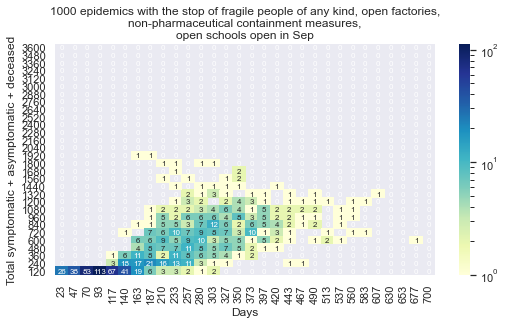
\includegraphics[width=0.8\textwidth]{HM30_readRunResults1k_with_NoAllFrag_openFacs_at20_openSchoolSep_plusHMlog.png}
\caption{Epidemics excluding fragility of any type, non-pharmaceutical containment measures, factories open, schools open in September 2020 (logarithmic scale for colors)}
\label{EpidemicsNoAllFragileFacsOnSchOnHM}
\end{center}
\end{figure}







\section{Appendix: How the visualization of contagion sequences works}
\label{appHowItWorks}

\subsection{The data}

With each new infection, we add a record to a file. Each record contains:
\begin{enumerate}\addtocounter{enumi}{-1}
\setlength{\itemsep}{0pt}
\item the ID of the agent transmitting the contagion (for the initial cases, externally generated, the ID has value -1);
\item its contagion progressive number, starting from 1 (for the initial cases, externally generated, this value is 0);
\item the conventional color of the place where it turned infected, following the NetLogo color swatches (for the externally generated initial cases, this value is 0);
\item the ID of the agent receiving the contagion;
\item its fragility rate (1 - robust; 2 - regular; 3 - fragile; 4 - extra fragile);
\item its contagion progressive number;
\item the conventional color of the place where it is turning infected, following the NetLogo color swatches;
\item the day (tick) of the contagion (for the initial cases, externally generated, this value is 0);
\item the starting infection day, i.e., the previous value plus the incubationPeriod (for the externally generated initial cases, the starting infection value is 0);
\item the day of the conclusion of the infection, i.e., the previous value plus a value between the minInfectionDuration and the maxInfectionDuration settings; this period stops if the agent deceases, but we do not consider that possibility here;
\item the symptomatic (1) or asymptomatic (2) status.
\end{enumerate}

\subsection{The plot}
\label{lineStyle}

Into the plots, each agent is represented by a horizontal line, starting at $x_1$ (date of the contagion, value 7 above) and finishing at $x_2$ (time of recover, value 9 above). 

The line is \emph{dotted} in the incubation phase (until value 8 above), then \emph{solid} for symptomatic cases or \emph{dashed} for asymptomatic ones. 

The line color is set by value 6 above. The line thickness is set by the value 4 above, with the scale: 1 robust, 2 regular, 3 fragile, 4 extra-fragile.

The position on y-axes is that of value 5 above. 

Using data 1, 2, 5 and 7, we plot a vertical line with: the contagion date as x position (value 7 above); the y1 position identifying the agent transmitting the contagion (value 1 above) and the y2 position identifying the agent receiving the contagion (value 5 above). The color is that of the transmitting agent.

Using  datum 4, we define the thickness of the horizontal lines : robust (lw = 1); regular (lw = 2); fragile (lw = 3); extra-fragile (lw = 4)

\subsection{The colors}
\begin{itemize}
\setlength{\itemsep}{0pt}
\item   black = contagion by an external unidentified agent;
\item    gray =  contagion in an empty or open space;
\item    orange = contagion in a nursing home;
\item    brown = contagion in a factory/office/shop;
\item    yellow = contagion in a school;
\item    cyan = contagion at home;
\item    pink = contagion in a hospital.
\end{itemize}


\section{Appendix: The calendar}
\label{appCalendar}

\begin{itemize}
\setlength{\itemsep}{0pt}

\item Day~1: conventionally, in the model the epidemic starts on Feb \nth{3}, 2020.

\item Day~17: due to carnival holidays, schools close.

\item Day~20: Piedmont Region first warning, with the prohibition of crowd gatherings.

\item Day~35: limitation of movement outside local areas.

\item Day~38: full lockdown on March \nth{11}.

\item Day~49: almost total blockage of non-essential production activities.

\item Day~84: reduction of the limitations.

\item Day~106: elimination of a large part of the restrictions; schools always inactive.

\end{itemize}


\bibliography{./bibliografiaGenerale}
\bibliographystyle{plainnatmm}

\end{document}  
